\deelzonderoef{Module 5}{Vergelijkingen, Ongelijkheden, Stelsels en Matrices}{Module 5. Vergelijkingen, Ongelijkheden, Stelsels en Matrices}

\section*{Intro}
\begin{minipage}{.25\linewidth}
	\raggedright
	
\includegraphics[width=4cm]{5_vglen_ongelijkheden_stelsels_matrices/inputs/QR_Code_INTRO_module5new}
\end{minipage}
\begin{minipage}{.7\linewidth}
	Zie filmpje MOOC.
\end{minipage}

\section{Vergelijkingen, ongelijkheden en stelsels}

\subsection*{Inleiding}

Het oplossen van vergelijkingen is een praktische wiskundige vaardigheid waarvan ondersteld wordt dat elke ingenieur ze beheerst. Op het eerste zicht lijkt vergelijkingen oplossen een spel met rare  regeltjes bedacht door wereldvreemde leraars wiskunde. Zodra je echter gaat narekenen of een voorgestelde technische oplossing voor een probleem eigenlijk wel mogelijk is, iets wat in het Engels heel toepasselijk wordt aangeduid als \textquotedblleft do the math\textquotedblright, behoort het oplossen van vergelijkingen tot de standaardactiviteiten.\\

Enkele voorbeelden:

\begin{itemize}

\item {In de thermodynamica speelt de toestandsvergelijking van een ideaal gas (in de volksmond \textquotedblleft de ideale gaswet\textquotedblright\ genoemd) een belangrijke rol. Deze vergelijking geeft voor een hoeveelheid (aantal mol $n$) ideaal gas het verband tussen druk $P$, temperatuur $T$ en volume $V$ bij thermisch evenwicht van het gas:

\[ PV=nRT \]

$R$ is een gekende constante.\\
Als het volume van de gasfles en de druk en temperatuur van het gas in de fles gekend zijn kan je de hoeveelheid gas in de fles berekenen door de vergelijking op te lossen naar de onbekende $n$.}

\item {Uit de fysica weten we dat een voorwerp dat op tijdstip $t=0$ op een hoogte $h_{0}$ wordt losgelaten zich na een valtijd $t$ op een hoogte $h$ zal bevinden gegeven door:

    \[ h(t)=h_{0}-\frac{1}{2}gt^2 \]

    Door de hoogte gelijk aan nul te stellen bekomt men de vergelijking:

    \[ h_{0}-\frac{1}{2}gt^2 =0 \]

    Oplossen van deze vergelijking naar de onbekende $t$ geeft de tijd die het voorwerp nodig heeft om de grond te bereiken.}

    \end{itemize}


\noindent Bij sommige toepassingen, zoals bijvoorbeeld het doorrekenen van elektrische netwerken, komt men meerdere vergelijkingen met meerdere onbekenden tegen waarvoor men een oplossing zoekt die moet voldoen aan alle vergelijkingen tegelijkertijd. In zo een geval spreekt men van het oplossen van een stelsel van vergelijkingen.\\

\subsection{Definities}

%\begin{itemize}
%	\item Wat is een vergelijking?
%    \item Wat is een onbekende?
%    \item Zijn er verschillende soorten vergelijkingen?
%	
%\end{itemize}

\begin{definitie}
	Een vergelijking drukt uit dat twee wiskundige uitdrukkingen aan elkaar gelijk zijn door een gelijkheidsteken tussen de uitdrukkingen te plaatsen.
\end{definitie}

\begin{voorbeeld}
	\[5x^3 + 2x = 8x^2 + 17\]
\end{voorbeeld}

De uitdrukking voor het gelijkheidsteken noemt met het linkerlid, de andere uitdrukking noemt men het rechterlid.\\

In een vergelijking staat altijd minstens \'{e}\'{e}n onbekende die met een letter wordt aangeduid. Dikwijls wordt hiervoor de letter $x$ gebruikt maar een onbekende kan met eender welke letter worden aangeduid. Het oplossen van een vergelijking komt erop neer dat je die waarden voor de onbekende (of onbekenden) zoekt waarvoor het linkerlid inderdaad gelijk is aan het rechterlid.

\begin{definitie}
	In deze nota's beperken we ons tot {\bf veeltermvergelijkingen}, dat zijn vergelijkingen waarbij zowel het rechterlid als het linkerlid veeltermen zijn, zoals in het voorbeeld hierboven.
\end{definitie} 

Er bestaan echter ook andere vergelijkingen. 

\begin{voorbeeld}
	De vergelijkingen

\[ 3\sin(x+2)=x^3 - 4x -1 \]

en

\[ \frac{1}{2} e^{-\pi y} - 4 = 37 \cos(y^2 +1) \]

zijn g\'{e}\'{e}n veeltermvergelijkingen.\\
\end{voorbeeld}

\begin{definitie}
	De {\bf graad van een veeltermvergelijking} is de hoogste macht van de onbekende die in de vergelijking voorkomt.
\end{definitie} De manier waarop men een veeltermvergelijking oplost is verschillend naargelang de graad van de vergelijking.\\
\begin{voorbeeld}
	

\[ 8t-2=0 \]

is een veeltermvergelijking van de eerste graad in de onbekende $t$, en

\[ h^{23} -2h^{12} + \frac{17}{3} h^7 + 4h^3 = \pi h -\frac{\pi}{2} \]

is een veeltermvergelijking van de $23$-ste graad in de onbekende $h$.\\

\end{voorbeeld}

\subsection{Eerstegraadsvergelijkingen}

We zullen het oplossen van eerstegraadsvergelijkingen verduidelijken met enkele voorbeelden.

%\subsubsection{Voorbeeld 1}

\begin{voorbeeld}

\[5x+3=3x+1\]

Het oplossen van de vergelijking komt er eigenlijk op neer dat je de vergelijking herschrijft op een zodanige manier dat je in \'{e}\'{e}n lid, en alleen daar, de onbekende hebt staan. Op die manier kan je de oplossing direct aflezen.
Het herschrijven van de vergelijking kan je doen door op het linkerlid en het rechterlid steeds dezelfde bewerkingen uit te voeren, op die manier blijft de gelijkheid tussen linkerlid en rechterlid gelden.\\
In bovenstaande vergelijking kunnen we van beide leden $3x$ aftrekken:

\[ 5x+3 \boldsymbol{-3x} = 3x +1 \boldsymbol{-3x} \]

dit geeft

\[ 2x+3 = 1 \]

Vervolgens trekken we van beide leden $3$ af:

\[ 2x+3 \boldsymbol{-3} = 1 \boldsymbol{-3} \]

dit geeft

\[ 2x = -2 \]

Om nu in het linkerlid alleen nog de onbekende over te houden kunnen we linkerlid en rechterlid delen door $2$:

\[ \frac{2x}{\boldsymbol{2}} = \frac{-2}{\boldsymbol{2}} \]

dit geeft

\[ x=-1 \]

als oplossing van de vergelijking.\\

\end{voorbeeld}

\begin{opmerking}
\ \\
\begin{itemize} \item Het uitvoeren van dezelfde optelling of aftrekking op het linker- en rechterlid komt erop neer  dat je termen van het ene lid naar het andere verplaatst. Hierbij moet je er wel op letten dat het teken van de term verandert bij overbrenging naar het andere lid. \item Het uitvoeren van dezelfde deling (of vermenigvuldiging) op linker- en rechterlid komt neer op het overbrengen van een factor naar het andere lid. Hierbij wordt een vermenigvuldiging een deling en omgekeerd. \item {Soms wordt de oplossing van een vergelijking genoteerd als een verzameling $S$. Voor het hierboven uitgewerkte voorbeeld schrijven we dan als oplossingenverzameling
 \[ S=\{-1\} \] }
\end{itemize}

\end{opmerking}

\begin{voorbeeld}

\[ 5y+4=5y-1  \]

We gaan opnieuw op dezelfde manier te werk. We kunnen bijvoorbeeld de term $5y$ uit het rechterlid overbrengen naar het linkerlid:

\[ 5y+4 \boldsymbol{-5y} = -1 \]

ofwel

\[ 4 = -1 \]

Dit is natuurlijk onzin!\\
Er is geen enkele waarde voor $y$ die ervoor kan zorgen dat $4=-1$, deze vergelijking heeft geen oplossingen...\\
Dit kan men ook noteren door te schrijven dat de oplossingenverzameling leeg is:

\[ S=\varnothing \]

\end{voorbeeld}

\begin{voorbeeld}

\[2(x-4)=7(3x-1)\]

De eerste stap is hier het uitwerken van de haakjes:
\[2(x-4)=7(3x-1) \Leftrightarrow 2x-8=21x-7\]
Vervolgens verplaatsen we de $-8$ naar rechts (min wordt plus):
\[2x=21x-7+8\Leftrightarrow 2x=21x+1\]
Nu verplaatsen we de $21x$ van rechts naar links (plus wordt min):
\[2x-21x=1\Leftrightarrow -19x=1\]
Dan brengen we $-19$ over naar het rechterlid (pas op: teken verandert niet!):
\[x=\frac{1}{-19}=-\frac{1}{19}\]

\end{voorbeeld}

\begin{ftonthoud}
	
Een goed stappenplan voor het oplossen van een eerstegraadsvergelijking is:
\begin{enumerate}
	\item Reken alle haakjes uit.
	\item Verplaats alle termen met onbekenden in naar een lid, alle termen zonder onbekenden naar het andere lid.
	       \begin{itemize}
                \item Elke bewerking die je links uitvoert, moet je rechts ook uitvoeren. \item Termen kan je overbrengen door het teken te veranderen: min wordt plus, plus wordt min. \item Factoren verplaats je door te delen of te vermenigvuldigen: een vermenigvuldiging wordt een deling en omgekeerd.
           \end{itemize}
\end{enumerate}
\end{ftonthoud}

\subsection{Oplossen van tweedegraadsvergelijkingen}

%\begin{itemize}
%		\item Hoeveel oplossingen heeft een tweedegraadsvergelijking?
%	    \item Hoe kan je die oplossingen vinden?
%\end{itemize}

Een tweedegraadsvergelijking wordt in de praktijk dikwijls vierkantsvergelijking of kwadratische vergelijking genoemd.

\subsubsection{Algemene methode om een tweedegraadsvergelijking op te lossen}

Een tweedegraadsvereglijking in de onbekende $x$ is een vergelijking van de vorm

\[ ax^2 + bx + c = 0 \]

met $a,b$ en $c$ re\"{e}le getallen, bovendien moet $a \neq 0$ zijn want anders hebben we een eerstegraadsvergelijking.\\
Om een dergelijke vergelijking op te lossen herschrijven we de vergelijking door ze te delen door $a$:

\[ x^2 + \frac{b}{a}x + \frac{c}{a} = 0 \]

Dit kan je ook schrijven als

\[ (x+ \frac{b}{2a})^2 + \frac{c}{a} - \frac{b^2}{4a^2} = 0 \]

Dit kan je controleren door de term met de haakjes uit te werken volgens het merkwaardige product $(A+B)^2 =A^2 + B^2 + 2AB $.\\
De term met de onbekende wordt nu naar het linkerlid verplaatst en de termen zonder de onbekende naar het rechterlid:

\[  (x+ \frac{b}{2a})^2 = \frac{b^2}{4a^2} - \frac{c}{a} \]

ofwel

\[ (x+ \frac{b}{2a})^2 = \frac{b^2 - 4ac}{4a^2} \]

Het berekenen van de vierkantswortel van linkerlid en rechterlid geeft

\[ x+\frac{b}{2a} = \frac{\sqrt{b^2 - 4ac}}{2a} \]

Dit is echter maar de helft van de oplossing. We zoeken immers die uitdrukkingen waarvan het kwadraat gelijk is aan $\frac{b^2 - 4ac}{4a^2}$, dit zijn zowel $+\frac{\sqrt{b^2 - 4ac}}{2a}$ als $-\frac{\sqrt{b^2 - 4ac}}{2a}$. Vergelijk dit bijvoorbeeld met $\sqrt{9}=3$ want $3^2 =9$, maar er geldt ook $(-3)^2 =9$ ... Als je dus de oplossingen zoekt van $y^2 =9$ geeft dit $y=3$ en $y=-3$. \\
We moeten dus rekening houden met de twee mogelijkheden:

\[ x+\frac{b}{2a} = + \frac{\sqrt{b^2 - 4ac}}{2a} \textup{  en  } x+\frac{b}{2a} = - \frac{\sqrt{b^2 - 4ac}}{2a} \]

Deze eestegraadsvergelijkingen oplossen naar $x$ geeft dan

\[ x_{1}=-\frac{b}{2a}+ \frac{\sqrt{b^2 - 4ac}}{2a} \textup{  en  } x_{2}=-\frac{b}{2a}- \frac{\sqrt{b^2 - 4ac}}{2a} \]

We vinden dus in principe {\bf twee oplossingen} voor een tweedegraadsvergelijking.\\
Merk op dat de uitdrukking onder de vierkantswortel, $b^2 - 4ac$, een belangrijke rol speelt. Als deze uitdrukking groter dan nul is hebben we twee verschillende re\"{e}le oplossingen, als deze uitdrukkig echter gelijk is aan nul dan zijn de twee oplossingen gelijk aan elkaar (praktisch gezien is er dan maar \'{e}\'{e}n  re\"{e}le oplossing), en als de uitdrukking kleiner is dan nul dan zijn er twee complexe oplossingen. Deze complexe oplossingen zijn bovendien elkaars complex toegevoegde. De tweedemachtswortels van een negatief re\"{e}el getal $z$ zijn immers $\sqrt{|z|}i$ en $-\sqrt{|z|}i$.\\
De uitdrukking $b^2 - 4ac$ maakt dus een onderscheid (discrimineert) tussen de verschillende soorten oplossingen die mogelijk zijn. Men noemt deze uitdrukking dan ook de {\bf discriminant}, meestal aangeduid met de Griekse hoofdletter delta $\Delta$ of soms ook met de hoofdletter $D$.\\

De algemene methode om een tweedegraadsvergelijking op te lossen kan dus worden samengevat als volgt:\\


\begin{ftonthoud}
	\ \\
	\begin{itemize}
\item Schrijf de vergelijking in de vorm $ax^2 + bx + c = 0$     ($a,b$ en $c$ re\"{e}le getallen)
\item Bereken de discriminant $\Delta = b^2 - 4ac$
\item Ga na hoeveel oplossingen er zijn:
        \begin{itemize} \item Als $\Delta >0$ dan zijn er $2$ verschillende re\"{e}le oplossingen \item Als $\Delta=0$ dan is er $1$ re\"{e}le oplossing (de $2$ oplossingen zijn gelijk aan elkaar) \item Als $\Delta <0$ dan zijn er twee complexe oplossingen die elkaars complex toegevoegde zijn \end{itemize}
\item De oplossingen worden gegeven door
\[ x_{1}=\frac{-b + \sqrt{\Delta}}{2a} \textup{  en  } x_{2}=\frac{-b - \sqrt{\Delta}}{2a} \]
Opmerking: In het geval dat $\Delta <0$ kan men (moet niet) de oplossingen ook schrijven als
\[ x_{1}=\frac{-b +i \sqrt{|\Delta|}}{2a} \textup{  en  } x_{2}=\frac{-b -i \sqrt{|\Delta|}}{2a} \]
\end{itemize}

\end{ftonthoud}

\begin{voorbeeld}
	

\[ x(4x+2)+4 = -3x+2 \]

We schrijven deze vergelijking in de standaardvorm $ax^2 +bx + c =0$:

\[ x(4x+2)+4 = -3x+2 \Leftrightarrow 4x^2 + 2x +4 = -3x +2 \Leftrightarrow 4x^2 + 5x +2 = 0 \]

Het symbool $\Leftrightarrow$ betekent zoveel als ``is equivalent met'' of ``als en slechts als''.\\
We berekenen nu de discriminant:

\[ \Delta = 5^2 - 4.4.2= 25-32= -7 \]

Aangezien $\Delta < 0$ zijn er twee copmlex toegevoegde complexe oplossingen:

\[ S= \frac{-5+i\sqrt{7}}{8}, -\frac{5+i\sqrt{7}}{8} \]

\end{voorbeeld}
\begin{voorbeeld}
	

\[ -4x^2 +5x +2=0 \]

We berekenen de discriminant:

\[ \Delta = 5^2 - 4.(-4).2 = 25 + 32 =57 \]

Er zijn dus twee verschillende oplossingen:

\[ x_{1}=\frac{-5 + \sqrt{57}}{2.(-4)} \textup{  en  } x_{2}=\frac{-5 - \sqrt{57}}{2.(-4)} \]

ofwel

\[ x_{1}=\frac{5 - \sqrt{57}}{8} \textup{  en  } x_{2}=\frac{5 + \sqrt{57}}{8} \]

De oplossingenverzameling is

\[ S=\{ \frac{5 - \sqrt{57}}{8}, \frac{5 + \sqrt{57}}{8} \} \] \\

\begin{opmerking}
	Slordig zijn met haakjes veroorzaakt fouten... Gebruik haakjes en respecteer de regels om met haakjes te werken!
\end{opmerking}

\end{voorbeeld}
\subsection{Speciale gevallen}

Elke vergelijking van de vorm $ax^2 +bx +c =0$ met $a \neq 0$ kan opgelost worden met de algemene methode met de discriminant. In sommige gevallen is het echter eenvoudiger om deze methode niet te gebruiken. We illustreren dit met enkele voorbeelden.


\begin{voorbeeld}
	
\[x^2=36\]

Dit is een tweedegraadsvergelijking in de meest eenvoudige vorm ($b=0$): in het linkerlid staat alleen een term met de onbekende en in het rechtermlid staat alleen een getal. Om de onbekende te vinden trekken we van beide leden de vierkantswortel:

\[ x=6 \]

Dit is zeker {\bf een} oplossing want $6^2 =36$. Maar er geldt ook dat $(-6)^2 =36$... Dus heeft de vergelijking nog een tweede oplossing:

\[ x=-6 \]

De oplossingen van de vergelijking zijn dus $x_{1}=+\sqrt{36}$ en $x_{2}=-\sqrt{36}$.\\
Met de oplossingenverzameling wordt dit genoteerd als

\[ S=\{ -6,6 \} \]

Uiteraard had je hier ook de algemene methode kunnen gebruiken.\\
Door de oorspronkelijke vergelijking in de standaardvorm te zetten vinden we:

\[ x^2 - 36 =0 \]

De discriminant is $\Delta= 0^2 - 4.1.(-36) = 144$.\\
De twee verschillende oplossingen zijn dan

\[ x_{1}=\frac{-0 + \sqrt{144}}{2.1} \textup{  en  } x_{2}=\frac{-0 - \sqrt{144}}{2.1} \]

ofwel

\[ x_{1}=6 \textup{  en  } x_{2}=-6 \]


\end{voorbeeld}


\begin{voorbeeld}
	\[3x^2=10x\]

We kunnen deze vergelijking oplossen door ze in de vorm $ax^2+bx+c=0$ te zetten:

\[3x^2-10x=0\]

Hier is dus $a=3$, $b=-10$ en $c=0$.\\
We berekenen de discriminat:

\[\Delta=(-10)^2-4\cdot 3 \cdot 0=100-0=100 \]

De twee oplossingen zijn dus:

\[ x_{1}=\frac{10+\sqrt{100}}{2.3} \textup{  en  } x_{2}=\frac{10-\sqrt{100}}{2.3} \]

ofwel

\[ x_{1}=\frac{10}{3} \textup{  en  } x_{2}=0 \]

Dit had echter veel eenvoudiger kunnen opgelost worden door de oorspronkelijke vergelijking te ontbinden in factoren:

\[3x^2-10x=0 \Leftrightarrow x(3x-10)=0  \]

De laatste vergelijking kan alleen maar nul zijn als $x=0$ of $3x-10=0$, met andere woorden de oplossingen zijn

\[ x_{1}=0 \textup{  en  } x_{2}=\frac{10}{3} \]

\end{voorbeeld}
\begin{voorbeeld}
	

\[ 17(x-1)(x+\pi)=0 \]

De kwadratische vergelijking is hier gegeven als een product van factoren waarin de onbekende $x$ lineair voorkomt. In dit geval is het {\bf niet } interessant om de haakjes uit te werken (het mag wel!). Het product kan alleen maar nul zijn als minstens \'{e}\'{e}n van de factoren nul is. Er is dus voldaan aan de vergelijking als $x-1=0$ of $x+\pi=0$.\\
De oplossingen zijn dus:

\[ x_{1}=1 \textup{  en  } x_{2}=-\pi \]

\end{voorbeeld}


Oplossen van tweedegraadsvergelijkingen:\\

\begin{ftonthoud}
	\ \\
\begin{itemize}
\item Schrijf de vergelijking in de vorm $ax^2 + bx + c = 0$ ($a,b$ en $c$ re\"{e}le getallen)
\item Bereken de discriminant $\Delta = b^2 - 4ac$
\item Ga na hoeveel oplossingen er zijn:
        \begin{itemize} \item Als $\Delta >0$ dan zijn er $2$ verschillende re\"{e}le oplossingen \item Als $\Delta=0$ dan is er $1$ re\"{e}le oplossing (de $2$ oplossingen zijn gelijk aan elkaar) \item Als $\Delta <0$ dan zijn er twee complexe oplossingen die elkaars complex toegevoegde zijn \end{itemize}
\item De oplossingen worden gegeven door
\[ x_{1}=\frac{-b + \sqrt{\Delta}}{2a} \textup{  en  } x_{2}=\frac{-b - \sqrt{\Delta}}{2a} \] 
Als $\Delta <0$ dan zijn er twee imaginaire oplossingen voor $\sqrt{\Delta}$: $i\sqrt{|\Delta|}$ en $-i\sqrt{|\Delta|}$ 
\end{itemize}

\begin{opmerking}
	Respecteer de rekenregels voor haakjes, voor het optellen en vermenigvuldigen van breuken, enz...  Denk niet dat je het sneller en beter kan op ``jouw manier''!
\end{opmerking}


\end{ftonthoud}

\subsection{Hogeregraadsvergelijkingen}

\subsubsection{Enkele nuttige weetjes over veeltermvergelijkingen in het algemeen}

Uit de theoretische algebra weet men dat:

\begin{itemize}
\item een veeltermvergelijking van de $n-$de graad met re\"{e}le co\"{e}ffici\"{e}nten $n$ complexe oplossingen heeft. Zo kan je op het zicht weten dat bijvoorbeeld de vergelijking $y^5 - \pi y^2 + 4y -28 = 0$ vijf complexe oplossingen heeft. Denk er aan dat een re\"{e}el getal ook een complex getal is!
\item een veeltermvergelijking met een oneven graad en re\"{e}le co\"{e}ffici\"{e}nten heeft altijd minstens \'{e}\'{e}n re\"{e}le oplossing (de vergelijking uit het voorbeeld heeft dus zeker $1$ re\"{e}le oplossing).
\item voor vergelijkingen van de derde en vierde graad bestaan er algemene oplossingsmethoden zoals voor tweedegraadsvergelijkingen (deze methoden zijn echter zeer langdradig en ingewikkeld en worden in de praktijk niet zoveel gebruikt).
\item voor vergelijkingen vanaf de vijfde graad bestaan er geen algemene theoretische oplossingsmethoden (dergelijke vergelijkingen worden numeriek opgelost, meestal met behulp van een computer of rekenmachine).
\end{itemize}

In een aantal speciale gevallen is het echter mogelijk om een hogeregraadsvergelijking toch met de hand op te lossen. Deze gevallen bespreken we hier.

\subsubsection{Substitutiemethode}

Sommige hogeregraadsvergelijkingen kunnen opgelost worden door een slimme substitutie.  Neem bijvoorbeeld de volgende vierdegraadsvergelijking:

\[x^4+3x^2-1=0\]

Door de substitutie $y=x^2$ toe te passen wordt deze vergelijking omgezet in een tweedegraadsvergelijking in de onbekende $y$.

\[ y^2+3y-1=0\]

Deze vergelijking kunnen we oplossen!\\
We berekenen de discriminant:

\[ \Delta= 3^2 - 4.1.(-1)=9+4=13 \]

Aangezien $\Delta >0$ zijn er $2$  verschillende oplossingen {\bf voor de tweedegraadsvergelijking}.

\[ y_{1}=\frac{-3 + \sqrt{13}}{2} \textup{  en  } y_{2}=\frac{-3 - \sqrt{13}}{2} \]

Dit zijn echter niet de oplossingen van de oorspronkelijke vierdegraadsvergelijking in de onbekende $x$. Het verband tussen de oplossingen van de vierdegraadsvergelijking en de waarden $y_{1}$ en $y_{2}$ wordt gegeven door de vergelijking $y=x^2$. We zoeken dus die waarden voor $x$ waarvoor het kwadraat $y_{1}$ en $y_{2}$ oplevert.

\[ x_{1}=\sqrt{\frac{-3 + \sqrt{13}}{2}} , x_{2}=-\sqrt{\frac{-3 + \sqrt{13}}{2}} , x_{3}=i\sqrt{\frac{3 + \sqrt{13}}{2}} , x_{4}=-i\sqrt{\frac{3 + \sqrt{13}}{2}}     \]

De oplossingenverzameling is

\[ S=\{ \sqrt{\frac{-3 + \sqrt{13}}{2}} , -\sqrt{\frac{-3 + \sqrt{13}}{2}} , i\sqrt{\frac{3 + \sqrt{13}}{2}} , -i\sqrt{\frac{3 + \sqrt{13}}{2}}  \} \]

\subsubsection{Ontbinden in factoren}

Beschouw de volgende derdegraadsvergelijking

\[ 5x^3-2x^2+3x = 0\]

Het linkerlid van deze vergelijking kunnen we schrijven als een product

\[ x(5x^2-2x+3)=0 \]

Aan deze vergelijking kan alleen maar voldaan worden als $x=0$ of $5x^2-2x+3=0$.\\
We hebben dus al \'{e}\'{e}n oplossing gevonden:

\[ x_{1}=0 \]

Om de eventuele andere oplossingen (maximaal drie) te vinden lossen we de vergelijking $5x^2-2x+3=0$ op.\\ We berekenen de discriminant: $\Delta = (-2)^2 - 4.5.3=4-60=-56 <0$. Er zijn dus twee complexe oplossingen voor $5x^2-2x+3=0$.\\

De oplossingenverzameling is

\[ S=\{ 0 , \frac{1+i\sqrt{14}}{5} , \frac{1-i\sqrt{14}}{5} \} \]

\begin{ftonthoud}
	Er bestaan geen algemene methoden om vergelijkingen van vijfde graad of hoger met de hand op te lossen. Deze methoden bestaan wel voor derdegraadsvergelijkingen en vierdegraadsvergelijkingen maar deze methoden zijn zeer omslachtig en worden daarom weinig gebruikt in de praktijk.\\

In een aantal speciale gevallen kunnen hogeregraadsvergelijkingen echter opgelost worden met \'{e}\'{e}n van de volgende technieken:
\begin{itemize}
	\item {\bf Substitutiemethode}
\begin{enumerate}
	\item Als de onbekende $x$ is vervang dan $x^2$ door een andere onbekende (zoals $y$) om een kwadratische vergelijking te bekomen.
	\item Los deze vergelijking op naar $y$.
	\item Los de vergelijkingen $y=x^2$ op naar de onbekende $x$.
\end{enumerate}

\item {\bf Ontbinden in factoren}
\begin{enumerate}
	\item Zet alle termen in het linkerlid zodat het rechterlid $0$ is.
	\item Ontbind het linkerlid in factoren door af te zonderen.
	\item De oplossingen worden gevonden door elke factor gelijk te stellen aan $0$.
\end{enumerate}
	
	
\end{itemize}

\begin{opmerking}
	Respecteer de rekenregels voor haakjes, voor het optellen en vermenigvuldigen van breuken, enz...
\end{opmerking}

\end{ftonthoud}


\subsection{Stelsels van vergelijkingen}
%
%\begin{itemize}
%	\item Wat is een stelsel van vergelijkingen?
%	\item Hoe kan men een eenvoudig stelsel van eerstegraadsvergelijkingen oplossen?
%\end{itemize}

\subsubsection{Inleiding}

\begin{definitie}
	Een stelsel van vergelijkingen bestaat uit minstens twee vergelijkingen in minstens twee onbekenden. Het bepalen van de onbekenden die tegelijkertijd oplossing zijn voor al de vergelijkingen van het stelsel noemt men het oplossen van het stelsel van vergelijkingen.
\end{definitie}

Als het stelsel van vergelijkingen alleen bestaat uit veeltermvergelijkingen van de eerste graad noemt men dit stelsel {\bf een lineair stelsel} of {\bf een stelsel van lineaire vergelijkingen}.\\ Een voorbeeld van een lineair stelsel van drie vergelijkingen in drie onbekenden $x$, $y$ en $z$:

\[\left\{ {
\begin{array}{l}
2x + 3y - 4z = 0\\
3x + 2y =  5\\
-x - 7y + z = -1
\end{array}} \right.\]

In de ingenieurswereld is het niet ongewoon om stelsels van tientallen vergelijkingen in tientallen onbekenden tegen te komen.\\


In de algebra toont men aan er voor een stelsel van eerstegraadsvergelijkkingen drie mogelijkheden zijn:
\begin{itemize}
\item Het stelsel is oplosbaar en heeft juist \'{e}\'{e}n oplossing.
\item Het stelsel is oplosbaar en heeft oneindig veel oplossingen.
\item Het stelsel heeft geen oplossingen.
\end{itemize}

In deze cursus beperken we ons tot het oplossen van stelsels van twee lineaire vergelijkingen. Voor dergelijke eenvoudige stelsels wordt gebruik gemaakt van de {\bf substitutiemethode}. \\

De substitutiemethode toegepast bij een stelsel van twee lineaire vergelijkingen werkt als volgt:
\begin{itemize}
\item Kies \'{e}\'{e}n van de vergelijking en los deze op naar \'{e}\'{e}n van de onbekenden, hierbij doe je net alsof je de andere onbekende kent.
\item Substitueer nu de oplossing van de ene vergelijking in de andere vergelijking, je bekomt nu een eerstegraadsvergelijking in \'{e}\'{e}n onbekende.
\item Los de bekomen vergelijking op en substitueer de gevonden onbekende in de andere vergelijking, dit levert een eerstegraadsvergelijking in de nog te vinden onbekende.
\item Los de overblijvende vergelijking op.
\item De gevonden oplossing(en) zijn oplossing voor allebei de vergelijkingen van het stelsel. Controleer dit door de waarden te substitueren!
\end{itemize}

We demonstreren de substitutiemethode met enkele voorbeelden.\\

\begin{voorbeeld}
	
\[\left\{ \begin{array}{l}
2x+y=0 \\
x-3y+1=0
\end{array} \right.\]

We kiezen bijvoorbeeld de eerste vergelijking en lossen deze op naar de onbekende $y$ waarbij we net doen alsof $x$ een gekend getal is:

\[ 2x+y=0 \Leftrightarrow y=-2x \]

We substitueren nu $y=-2x$ in de tweede vergelijking en lossen de nieuwe vergelijking op naar $x$:

\[ x-3(-2x)+1=0 \Leftrightarrow x+6x+1=0 \Leftrightarrow 7x+1=0 \Leftrightarrow x=-\frac{1}{7} \]

We substitueren de gevonden $x$ nu terug in de eerste vergelijking $y=-2x$:

\[ y=-2(-\frac{1}{7}) \Leftrightarrow y=\frac{2}{7} \]

De oplossing voor het stelsel is dus

\[ \left\{ \begin{array}{l}
x=-\frac{1}{7} \\
y=\frac{2}{7}
\end{array} \right. \]

Controle door deze waarden voor $x$ en $y$ in het oorspronkelijke stelsel te substitueren:

\[ \left\{ \begin{array}{l}
2(-\frac{1}{7})+\frac{2}{7}=0 \\
-\frac{1}{7}-3(\frac{2}{7})+1=0
\end{array} \right.\]

\end{voorbeeld}
\begin{voorbeeld}
	

\[\left\{ \begin{array}{l}
3x + 2y = 4\\
2x - 3y = 22
\end{array} \right.\]

Soms wordt om de zaken overzichtelijk te houden bij elke stap het volledige stelsel opnieuw opgeschreven. Dit vraagt heel wat extra schrijfwerk maar het kan wel helpen om fouten te vermijden.\\
We kiezen bijvoorbeeld de eerste vergelijking en lossen deze op naar $x$:

\[\left\{ \begin{array}{l}
3x + 2y = 4 \\
2x - 3y = 22
\end{array} \right. \Leftrightarrow \left\{ \begin{array}{l}
3x = 4 - 2y\\
2x - 3y = 22
\end{array} \right. \Leftrightarrow \left\{ \begin{array}{l}
x = \frac{4 - 2y}{3}\\
2x - 3y = 22
\end{array} \right.\]

Vervolgens substitueren we

\[x = \frac{4 - 2y}{3} \]

in de tweede vergelijking:

\[ \left\{ \begin{array}{l}
x = \frac{4 - 2y}{3}\\
2 ( \frac{4 - 2y}{3} ) - 3y = 22
\end{array} \right.\]

Dit geeft dan:

\[\left\{ \begin{array}{l}
x = \frac{4 - 2y}{3} \\
\frac{2.4}{3} -\frac{2.2}{3}y -3y = 22
\end{array} \right. \Leftrightarrow \left\{ \begin{array}{l}
x = \frac{4 - 2y}{3}\\
\frac{8}{3}-\frac{4}{3}y -3y = 22
\end{array} \right.\]

en

\[\left\{ \begin{array}{l}
x = \frac{4 - 2y}{3} \\
\frac{-4-9}{3}y = \frac{66-8}{3}
\end{array} \right. \Leftrightarrow \left\{ \begin{array}{l}
x = \frac{4 - 2y}{3}\\
-13y=58
\end{array} \right.\]

dus

\[y=-\frac{58}{13} \]

Dit substitueren we nu in de eerste vergelijking:

\[\left\{ \begin{array}{l}
x = \frac{4 - 2(-\frac{58}{3})}{3} \\
y=-\frac{58}{3}
\end{array} \right. \Leftrightarrow \left\{ \begin{array}{l}
x = \frac{4+\frac{116}{13}}{3}\\
y=-\frac{58}{13}
\end{array} \right.\]

Uitwerken geeft:

\[\left\{ \begin{array}{l}
x = \frac{\frac{52+116}{13}}{3} \\
y=-\frac{58}{13}
\end{array} \right. \Leftrightarrow \left\{ \begin{array}{l}
x = \frac{56}{13}\\
y=-\frac{58}{13}
\end{array} \right.\]

Controleer zelf de correctheid van de gevonden oplossing door $x$ en $y$ te substitueren in het oorspronkelijke stelsel van vergelijkingen.\\

\begin{opmerking}
	Hopelijk heb je gemerkt dat het zo goed als onmogelijk is dergelijke berekeningen uit te voeren zonder op een correcte manier met de rekenregels voor haakjes en breuken om te springen...
\end{opmerking}

\end{voorbeeld}

\begin{voorbeeld}
	
\[\left\{ \begin{array}{l}
\pi x - 5y = 0\\
2 \pi x - 10y = \frac{\pi}{17}
\end{array} \right.\]

De eerste vergelijking oplossen naar $x$ geeft:

\[ x=\frac{5}{\pi}y \]

Dit substitueren in de tweede vergelijking en uitwerken geeft:

\[\left\{ \begin{array}{l}
x=\frac{5}{\pi}y \\
2 \pi (\frac{5}{\pi}y) - 10y = \frac{\pi}{17}
\end{array} \right. \Leftrightarrow \left\{ \begin{array}{l}
x=\frac{5}{\pi}y \\
10y -10y = \frac{\pi}{17}
\end{array} \right. \Leftrightarrow \left\{ \begin{array}{l}
x=\frac{5}{\pi}y \\
0=\frac{\pi}{17}
\end{array} \right.\]

De tweede vergelijking van het stelsel is duidelijk onzin, er bestaat geen $x$ en $y$ die ervoor kan zorgen dat deze vergelijking klopt.\\

{\bf Het stelsel van vergelijkingen heeft geen oplossingen!}

\end{voorbeeld}

\begin{voorbeeld}
	

\[\left\{ \begin{array}{l}
84x-210y=21\\
2x-5y = \frac{1}{2}
\end{array} \right.\]

We lossen de tweede vergelijking op naar $y$:

\[ 2x-5y = \frac{1}{2} \Leftrightarrow \frac{2x-\frac{1}{2}}{5}=y \Leftrightarrow y=\frac{4x-1}{10} \]

Substitutie in de eerste vergelijking geeft dan

\[\left\{ \begin{array}{l}
84x-210(\frac{4x-1}{10})=21 \\
y=\frac{4x-1}{10}
\end{array} \right. \Leftrightarrow \left\{ \begin{array}{l}
84x-84x+21=21 \\
y=\frac{4x-1}{10}
\end{array} \right. \Leftrightarrow \left\{ \begin{array}{l}
21=21\\
y=\frac{4x-1}{10}
\end{array} \right.\]

Hier zien we dat de eerste vergelijking altijd geldig is, welke waarden voor $x$ en $y$ men ook kiest.\\
Alleen de tweede vergelijking legt beperkingen op aan $x$ en $y$, namelijk dat om een oplossing van het stelsel te hebben het verband tussen $x$ en $y$ moet gegeven worden door

\[ y=\frac{4x-1}{10} \]

Je kan dus ofwel $x$, ofwel $y$ willekeurig kiezen. Als je de andere onbekende berekent met de tweede vergelijking zijn $x$,$y$ een oplossing voor het stelsel.\\

{\bf Dit betekent dat het stelsel een oneindig aantal oplossingen heeft!} \\

De oplossingen worden gegeven door

\[\left\{ \begin{array}{l}
x \in \mathbb{R} \\
y=\frac{4x-1}{10}
\end{array} \right. \]


\end{voorbeeld}

\begin{ftonthoud}
	
\begin{itemize}
\item Kies \'{e}\'{e}n van de vergelijking en los deze op naar \'{e}\'{e}n van de onbekenden, hierbij doe je net alsof je de andere onbekende kent.
\item Substitueer nu de oplossing van de ene vergelijking in de andere vergelijking, je bekomt nu een eerstegraadsvergelijking in \'{e}\'{e}n onbekende.
\item Los de bekomen vergelijking op en substitueer de gevonden onbekende in de andere vergelijking, dit levert een eerstegraadsvergelijking in de nog te vinden onbekende.
\item Los de overblijvende vergelijking op.
\item De gevonden oplossing(en) zijn oplossing voor allebei de vergelijkingen van het stelsel. Controleer dit door de waarden te substitueren!
\end{itemize}

\begin{opmerking}
	Respecteer de rekenregels voor haakjes, voor het optellen en vermenigvuldigen van breuken, enz...
\end{opmerking}
\end{ftonthoud}


Tips:
\begin{framed}
\begin{itemize}
	\item Let goed op bij substitutie dat je de hele uitdrukking substitueert, gebruik haakjes!
	\item Je mag een vergelijking apart afhandelen, maar vergeet niet op het einde alles terug in het stelsel te zetten!
\end{itemize}
\end{framed}

\subsection{Ongelijkheden}

%\begin{itemize}
%\item Wat is een ongelijkheid?
%\item Hoeveel oplossingen zijn er voor een ongelijkheid en hoe kan je die vinden?
%\end{itemize}

\subsubsection{Inleiding}

Men bekomt een ongelijkheid door in een vergelijking het ``is gelijk aan'' teken te vervangen door \'{e}\'{e}n van de volgende ongelijkheidstekens:
\begin{itemize}
\item $ < $ ``is kleiner dan''
\item $ > $  ``is groter dan''
\item $ \leq $ ``is kleiner dan of gelijk aan''
\item $ \geq $ ``is groter dan of gelijk aan''
\end{itemize}

Je kan ongelijkheden op een soortgelijke manier manipuleren als vergelijkingen.
\begin{itemize}
\item Door bij het linkerlid en rechterlid van een ongelijkheid hetzelfde positieve of negatieve getal op te tellen blijft de ongelijkheid geldig. Door bijvoorbeeld in beide leden van de ongelijkheid $x+1>8$ het getal $2$ op te tellen vinden we $x+3>10$ en door het getal $2$ af te trekken bekomt men $x-1>6$. Dit zijn drie equivalente ongelijkheden met dezelfde oplossingen: $x>7$.
\item Door beide leden van een ongelijkheid met hetzelfde (van nul verschillende) positieve getal te vermenigvuldigen bekomt men een equivalente ongelijkheid, door bijvoorbeeld $x+1>8$ te vermenigvuldigen met $10$ bekomt men $10x+10>80$ met nog steeds dezelfde oplossingen $x>7$.
\item {\bf Pas op!} Als men een ongelijkheid vermenigvuldigt met een negatief getal dan keert het ongelijkheidsteken om! Nemen we weer hetzelfde voorbeeld $x+1>8$ en vermenigvuldigen we deze uitdrukking met $-1$ dan bekomen we $-x-1<-8$. Alleen op deze manier blijven de oplossingen hetzelfde: $x>7$.
\end{itemize}

In deze cursus zullen we met behulp van een aantal voorbeelden illustreren hoe men ongelijkheden van de eerste graad kan oplossen.\\

\begin{voorbeeld}
	

\[ 5x-7 < 2x+1 \]

Door bij beide leden $2x$ af te trekken en $7$ bij te tellen vinden we

\[ 3x<8 \]

Delen door $3$ geeft

\[ x< \frac{8}{3} \]

Deze ongelijkheid heeft dus oneindig veel oplossingen!

Deze oplossingen worden soms ook genoteerd met de oplossingenverzameling:

\[ S=] -\infty, \frac{8}{3} [ \]

Met deze notatie wordt de verzameling van alle getallen tussen $-\infty$ en $\frac{8}{3}$ aangegeven, merk op dat $-\infty$ en $\frac{8}{3}$ niet tot de oplossingenverzameling behoren (dit wordt aangegeven door de naar buiten wijzende vierkante haakjes).

\end{voorbeeld}
\begin{voorbeeld}
	

\[ 5x-7 < 8x+1 \]

Door bij beide leden $8x$ af te trekken en $7$ bij te tellen vinden we

\[ -3x<8 \]

Delen door $-3$ geeft

\[ x> -\frac{8}{3} \]

Let op! Het ``$<$''-teken wordt het ``$>$''-teken!\\

De oplossingenverzameling wordt genoteerd als

\[ S=]-\frac{8}{3}, +\infty [ \]

\end{voorbeeld}
\begin{voorbeeld}
	

\[ 17x+7 \geq 17x+3\pi \]

Van beide leden $17x$ aftrekken geeft

\[ 7 \geq 3 \pi \]

Er is geen enkele $x$ die ervoor kan zorgen dat hieraan voldaan is. Deze ongelijkheid heeft geen oplossingen. De oplossingenverzameling is leeg:

\[ S=\varnothing \]


\end{voorbeeld}
\begin{voorbeeld}
	

\[ \frac{x}{3}+1 \leq -\frac{5}{7}x-12 \]

Vermenigvuldigen met $3$ geeft

\[ x+3 \leq -\frac{15}{7}x-36 \]

Het wegwerken van de term met $x$ in het rechterlid en de constante term in het linkerlid geeft

\[ \frac{22}{7}x \leq -39 \]

Vermenigvuldigen met $\frac{7}{22}$ geeft tenslotte

\[ x \leq -\frac{273}{22} \]

De oplossingenverzameling is

\[ S=]-\infty, -\frac{273}{22} ] \]

Merk op dat het naar binnen wijzende vierkante haakje aanduidt dat $-\frac{273}{22}$ wel degelijk tot de oplossingenverzameling behoort.

\end{voorbeeld}

\begin{ftonthoud}
	\ \\
	\begin{itemize}
\item Ongelijkheden van de eerste graad lost men op door de onbekende af te zonderen op een soortgelijke manier als bij veeltermvergelijkingen van de eerste graad.
\item Let op dat bij het vermenigvuldigen van de ongelijkheid met een negatief getal ``groter dan (of gelijk aan)'' wordt omgezet in ``kleiner dan (of gelijk aan)'' en omgekeerd.
\item Een ongelijkheid heeft ofwel oneindig veel oplossingen ofwel geen oplossingen.
\end{itemize}
\end{ftonthoud}


\section{Matrices}

\subsection*{Inleiding}

Stel dat je een computerspel speelt en je op een beeldscherm, of eventueel door een virtual reality headset, naar een door een computer gegenereerd landschap kijkt. Kijk je in deze wereld een beetje naar links of naar rechts dan berekent de computer hoe het landschap eruit ziet in je nieuwe kijkrichting en je ziet de virtuele wereld als het ware rond je gezichtspunt roteren. Misschien heb je er nog niet bij stilgestaan maar bij dit soort zaken wordt stevig gebruikt gemaakt van wiskunde.\\
We kunnen een idee krijgen van hoe dit in zijn werk gaat door ons in eerste instantie te beperken tot een twee dimensionale situatie. In de figuur is een punt $P$ voorgesteld waarvan de positie in het vlak is vastgelegd door een plaatsvector $\vec{r}$. Deze plaatsvector kan voorgesteld worden ten opzichte van verschillende basissen. 

%\begin{figure}[h]
%	\begin{center}
%		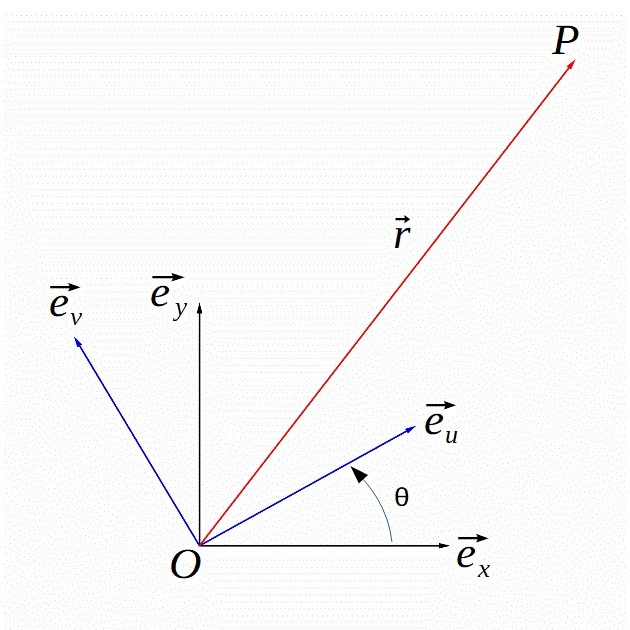
\includegraphics[scale=0.5]{5_vglen_ongelijkheden_stelsels_matrices/inputs/matrices-fig-1}
%	\end{center}
%\end{figure}

\begin{center}
\begin{tikzpicture}

\coordinate (a) at (0,0) node[anchor=south,below,xshift=-0.3cm]{$O$};
\coordinate (b) at (0.866,0.5);
\coordinate (c) at (0.866,0);

\draw[thin,gray!40] (-3,-1) (3,3);
\draw[->] (-3,0)--(3,0) node[right]{$x$};
\draw[->] (0,-1)--(0,3) node[above]{$y$};
\draw[line width=2pt,black,-stealth](0,0)--(2,0) node[anchor=south,xshift=0.3cm]{$\vec{e_x}$};
\draw[line width=2pt,black,-stealth](0,0)--(0,2) node[anchor=south,xshift=0.3cm]{$\vec{e_y}$};

%\draw[red] node[]{$P$}

\draw[line width=2pt,blue,-stealth](0,0)--(1.732,1) node[anchor=south]{$\vec{e_u}$};
\draw[line width=2pt,blue,-stealth](0,0)--(-1,1.732) node[anchor=south]{$\vec{e_v}$};

\draw[line width=2pt,red,-stealth](0,0)--(2.5,3) node[anchor=south,above, midway]{$\vec{r}$} node[anchor=south]{$P$};

%\path[clip] (0.866,0.5) -- (0,0) -- (0.866,0) -- cycle;
%\node[circle,draw=black,minimum size=40pt] at (0,0) (circ) {};
%\draw[blue] (1cm,0cm) arc (90:125:0.5cm);

%  \draw
%(3,-1) coordinate (a) node[right] {a}
%-- (0,0) coordinate (b) node[left] {b}
%-- (2,2) coordinate (c) node[above right] {c}
%pic["$\alpha$",draw=orange,<->,angle eccentricity=1.2,angle radius=1cm] {angle=a--b--c};

\pic [draw, -, "$\theta$", angle eccentricity=1.5] {angle = c--a--b};


%\draw[line width=2pt,blue,-stealth](0,0)--(-0.5,$\sqrt{3}/2$) node[anchor=south]{$\vec{e_v}$};

\end{tikzpicture}
\end{center}

In de figuur worden twee orthonormale basissen (m.a.w. basissen van loodrecht op elkaar staande \'{e}\'{e}nheidsvectoren) gebruikt waarbij de basis $\{\vec{e}_u ,\vec{e}_v \}$ over een hoek $\theta$ is geroteerd ten opzichte van de basis $\{\vec{e}_x ,\vec{e}_y \}$. \\  De plaatsvector van het punt $P$ wordt ten opzichte van de basis $\{\vec{e}_x ,\vec{e}_y \}$ geschreven als

\[  \vec{r}=x \vec{e}_x + y \vec{e}_y \] 

en ten opzichte van de basis $\{\vec{e}_u ,\vec{e}_v \}$ als 

\[  \vec{r}=u \vec{e}_u + v \vec{e}_v \] 

Om te beschrijven wat er gebeurt bij een rotatie van ons referentiestelsel over een hoek $\theta$ moeten we het verband vinden tussen de co\"{o}rdinaten van het punt $P$ in de twee referentiestelsels, met andere woorden we moeten het verband vinden tussen de componenten van $\vec{r}$ ten opzichte van de basis $\{\vec{e}_u ,\vec{e}_v \}$ en ten opzichte van de basis $\{\vec{e}_x ,\vec{e}_y \}$.\\ 

Door te projecteren kunnen we de componenten van de \'{e}\'{e}nheidsvectoren van de basis $\{\vec{e}_u ,\vec{e}_v \}$ schrijven ten opzichte van de basis $\{\vec{e}_x ,\vec{e}_y \}$.

\[  
\left \{ \begin{array}{l} 
\vec{e}_u =\cos \theta \vec{e}_x + \sin \theta \vec{e}_y \\
\vec{e}_v =-\sin \theta \vec{e}_x + \cos \theta \vec{e}_y
\end{array}  \right.
\]

Omgekeerd kunnen we de componenten van de basisvectoren $\{\vec{e}_x ,\vec{e}_y \}$ ten opzichte van de basis $\{\vec{e}_u ,\vec{e}_v \}$ neerschrijven als volgt:

\[  
\left \{ \begin{array}{l} 
\vec{e}_x =\cos \theta \vec{e}_u - \sin \theta \vec{e}_v \\
\vec{e}_y =\sin \theta \vec{e}_u + \cos \theta \vec{e}_v
\end{array}  \right.
\]

Door substitutie in $\vec{r}=u \vec{e}_u + v \vec{e}_v$ vinden we

\[ \vec{r}=u(\cos \theta \vec{e}_x + \sin \theta \vec{e}_y) + v(-\sin \theta \vec{e}_x + \cos \theta \vec{e}_y)  \]

ofwel

\[ \vec{r}=(u \cos \theta -v \sin \theta)\vec{e}_x + (u \sin \theta + v \cos \theta)\vec{e}_y \]

De co\"{o}rdinaten van het punt $P$ in het oorspronkelijke referentiestelsel worden dus als volgt geschreven in functie van de co\"{o}rdinaten van het punt $P$ in het nieuwe referentiestelsel:

\[   
\left\{ \begin{array}{l}
x= u \cos \theta -v \sin \theta \\
y= u \sin \theta + v \cos \theta \end{array} \right.
\]

Op dezelfde manier vindt men door substitutie de co\"{o}rdinaten van het punt $P$ in het nieuwe referentiestelsel, uitgedrukt in functie van de co\"{o}rdinaten van $P$ in het oude referentiestelsel:

\[   
\left\{ \begin{array}{l}
u= x \cos \theta + y \sin \theta \\
v= -x \sin \theta + y \cos \theta \end{array} \right.
\]

Deze uitdrukkingen kan men ook op een alternatieve, elegante manier neerschrijven met behulp van getallenschema's. De co\"{o}rdinaten in een referentiestelsel schrijft met in een kolom, een {\bf kolommatrix} en het verband tussen de co\"{o}rdinaten in beide referentiestelsels drukt met uit met een {\bf co\"{o}rdinatentransformatiematrix}.

\[
\left( \begin{array}{l} u \\ v \end{array} \right)= \left( \begin{array}{rr} \cos \theta & \sin \theta \\ -\sin \theta & \cos \theta \end{array} \right) \left( \begin{array}{l} x \\ y \end{array} \right) 
\]

Een soortgelijke, maar verschillende situatie wordt in de volgende figuur voorgesteld. Een vector $\vec{r}=x \vec{e}_x + y \vec{e}_y$ roteert over een hoek $-\theta$ (dus gemeten in wijzerszin), na deze rotatie wordt de vector, die we nu $\vec{r'}$ noemen, gegeven door $\vec{r'}$=$x' \vec{e}_x + y' \vec{e}_y$. 

\begin{center}
	\begin{tikzpicture}
	
	\coordinate (a) at (0,0) node[anchor=south,below,xshift=-0.3cm]{$O$};
	\coordinate (b) at (3.66,1.35);
	\coordinate (c) at (2.5,3);
	
	\draw[thin,gray!40] (-3,-1) (3,3);
	\draw[->] (-3,0)--(3,0) node[right]{$x$};
	\draw[->] (0,-1)--(0,3) node[above]{$y$};
	\draw[line width=2pt,black,-stealth](0,0)--(2,0) node[anchor=south,xshift=0.3cm]{$\vec{e_x}$};
	\draw[line width=2pt,black,-stealth](0,0)--(0,2) node[anchor=south,xshift=0.3cm]{$\vec{e_y}$};
	
%	\draw[line width=2pt,blue,-stealth](0,0)--(1.732,1) node[anchor=south]{$\vec{e_u}$};
%	\draw[line width=2pt,blue,-stealth](0,0)--(-1,1.732) node[anchor=south]{$\vec{e_v}$};
	
	\draw[line width=2pt,red,-stealth](0,0)--(2.5,3) node[anchor=south,above, midway]{$\vec{r}$} node[anchor=south]{$P$};
	
	\draw[line width=2pt,blue,-stealth](0,0)--(3.66,1.35) node[anchor=south,above, midway]{$\vec{r'}$} node[anchor=south]{$P'$};
	
	%\path[clip] (0.866,0.5) -- (0,0) -- (0.866,0) -- cycle;
	%\node[circle,draw=black,minimum size=40pt] at (0,0) (circ) {};
	%\draw[blue] (1cm,0cm) arc (90:125:0.5cm);
	
	%  \draw
	%(3,-1) coordinate (a) node[right] {a}
	%-- (0,0) coordinate (b) node[left] {b}
	%-- (2,2) coordinate (c) node[above right] {c}
	%pic["$\alpha$",draw=orange,<->,angle eccentricity=1.2,angle radius=1cm] {angle=a--b--c};
	
	\pic [draw, <-, "$-\theta$", angle eccentricity=2] {angle = b--a--c};
	
	
	%\draw[line width=2pt,blue,-stealth](0,0)--(-0.5,$\sqrt{3}/2$) node[anchor=south]{$\vec{e_v}$};
	
	\end{tikzpicture}
\end{center}

%\begin{figure}[h]
%	\begin{center}
%		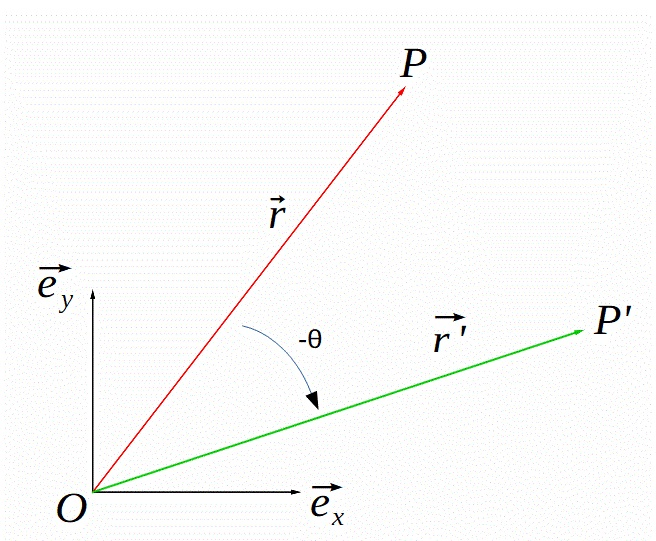
\includegraphics[scale=0.5]{5_vglen_ongelijkheden_stelsels_matrices/inputs/matrices-fig-2}
%	\end{center}
%\end{figure}

De componenten van $\vec{r'}$ worden nu uitgedrukt in functie van de componenten van $\vec{r}$ met

\[
\left( \begin{array}{l} x' \\ y' \end{array} \right)= \left( \begin{array}{rr} \cos \theta & \sin \theta \\ -\sin \theta & \cos \theta \end{array} \right) \left( \begin{array}{l} x \\ y \end{array} \right) 
\]

In de volgende figuur is de rotatie van een vector $\vec{r}$ over een hoek $\theta$ in tegenwijzerszin voorgesteld.

\begin{center}
	\begin{tikzpicture}
	
	\coordinate (a) at (0,0) node[anchor=south,below,xshift=-0.3cm]{$O$};
	\coordinate (b) at (3.66,1.35);
	\coordinate (c) at (2.5,3);
	
	\draw[thin,gray!40] (-3,-1) (3,3);
	\draw[->] (-3,0)--(3,0) node[right]{$x$};
	\draw[->] (0,-1)--(0,3) node[above]{$y$};
	\draw[line width=2pt,black,-stealth](0,0)--(2,0) node[anchor=south,xshift=0.3cm]{$\vec{e_x}$};
	\draw[line width=2pt,black,-stealth](0,0)--(0,2) node[anchor=south,xshift=0.3cm]{$\vec{e_y}$};
	
	%	\draw[line width=2pt,blue,-stealth](0,0)--(1.732,1) node[anchor=south]{$\vec{e_u}$};
	%	\draw[line width=2pt,blue,-stealth](0,0)--(-1,1.732) node[anchor=south]{$\vec{e_v}$};
	
	\draw[line width=2pt,red,-stealth](0,0)--(3.66,1.35) node[anchor=south,above, midway]{$\vec{r}$} node[anchor=south]{$P$};
	
	\draw[line width=2pt,blue,-stealth](0,0)--(2.5,3) node[anchor=south,above, midway]{$\vec{r'}$} node[anchor=south]{$P'$};
	
	%\path[clip] (0.866,0.5) -- (0,0) -- (0.866,0) -- cycle;
	%\node[circle,draw=black,minimum size=40pt] at (0,0) (circ) {};
	%\draw[blue] (1cm,0cm) arc (90:125:0.5cm);
	
	%  \draw
	%(3,-1) coordinate (a) node[right] {a}
	%-- (0,0) coordinate (b) node[left] {b}
	%-- (2,2) coordinate (c) node[above right] {c}
	%pic["$\alpha$",draw=orange,<->,angle eccentricity=1.2,angle radius=1cm] {angle=a--b--c};
	
	\pic [draw, ->, "$\theta$", angle eccentricity=2] {angle = b--a--c};
	
	
	%\draw[line width=2pt,blue,-stealth](0,0)--(-0.5,$\sqrt{3}/2$) node[anchor=south]{$\vec{e_v}$};
	
	\end{tikzpicture}
\end{center}


%\begin{figure}[h]
%	\begin{center}
%		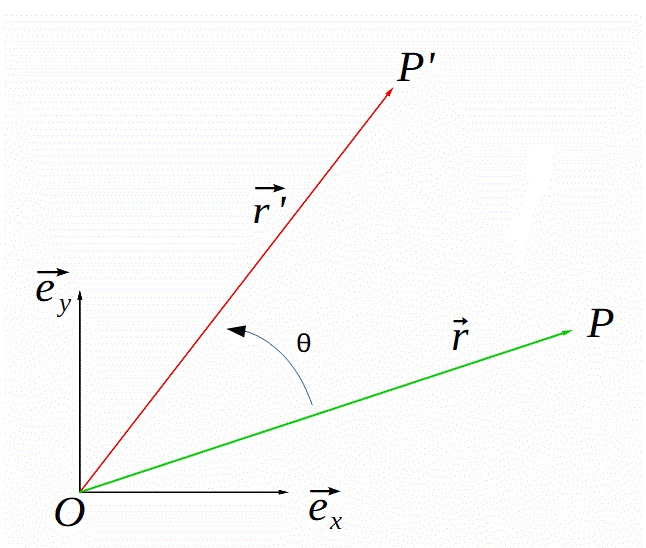
\includegraphics[scale=0.5]{5_vglen_ongelijkheden_stelsels_matrices/inputs/matrices-fig-3}
%	\end{center}
%\end{figure}

De transformatie voor deze rotatie vinden we door in de bovenstaande uitdrukking $\theta$ te vervangen door $-\theta$. We vinden dan:

\[
\left( \begin{array}{l} x' \\ y' \end{array} \right)= \left( \begin{array}{rr} \cos \theta & -\sin \theta \\ \sin \theta & \cos \theta \end{array} \right) \left( \begin{array}{l} x \\ y \end{array} \right) 
\]

De matrix

\[
\left( \begin{array}{rr} \cos \theta & -\sin \theta \\ \sin \theta & \cos \theta \end{array} \right)
\]

wordt de rotatiematrix voor rotatie over een hoek $\theta$ genoemd.\\

Matrices zijn een handige manier om veranderingen van referentiestelsel, co\"{o}rdinatentransformaties, te beschrijven.\\
Daarnaast is er een hele familie bewerkingen, lineaire transformaties, waarbij een vector via een matrixbewerking wordt omgezet in een nieuwe vector. Typisch voorbeeld is het roteren van een vector zoals hierboven beschreven.\\

In dit hoofdstuk zullen we een aantal definities en eigenschappen van matrices bespreken en zullen we rekenwerk met matrices inoefenen met het oog op praktische toepassingen. Alle eigenschappen die besproken worden kunnen wiskundig bewezen worden maar dat gaan we in dit hoofdstuk dus niet doen.\\

\newpage

\subsection{Definities}

%\begin{itemize}
%	\item Wat is een matrix?
%    \item Welke bewerkingen zijn er mogelijk met matrices?
%    \item Wat hebben matrices te maken met het oplossen van stelsels van vergelijkingen?
%\end{itemize}

\subsubsection{Definitie van een matrix}

\begin{definitie}
	Een $m \times n$ matrix $A$ is een rechthoekig getallenschema waarin re\"{e}le en/of complexe getallen in $m$ rijen en $n$ kolommen zijn gerangschikt. Het getal op de $i$-de rij en $j$-de kolom wordt symbolisch weergegeven als $a_{ij}$.

\end{definitie}
\[
A= \left( \begin{matrix}
a_{11} & a_{12} & a_{13} & \ldots & a_{1n} \\
a_{21} & a_{22} & a_{23} & \ldots & a_{2n} \\
\vdots & \vdots & \vdots & \ddots & \vdots \\
a_{m1} & a_{m2} & a_{m3} & \ldots & a_{mn}
\end{matrix} \right)
\]

\subsubsection{Enkele veel voorkomende speciale matrices}

\begin{itemize}
\item{Een rijmatrix}

Een matrix $A$ met $1$ rij en $n$ kolommen wordt een $1xn$ matrix of rijmatrix genoemd.

\[
A= \left( \begin{matrix}
a_{11} & a_{12} & a_{13} & \ldots & a_{1n}
\end{matrix} \right)
\]

\item{Een kolommatrix}

Een matrix $A$ met $m$ rijen en $1$ kolom wordt een $mx1$ matrix of kolommatrix genoemd.

\[
A= \left( \begin{matrix}
a_{11} \\
a_{21} \\
a_{31} \\
\vdots \\
a_{m1}
\end{matrix} \right)
\]

\item{Een vierkante matrix}

Een matrix met evenveel rijen als kolommen wordt een vierkante matrix genoemd.\\ De onderstaande matrix $A$ is een $n \times n$ matrix.

\[
A= \left( \begin{matrix}
a_{11} & a_{12} & \ldots & a_{1n} \\
a_{21} & a_{22} & \ldots & a_{2n} \\
\vdots & \vdots & \ddots & \vdots \\
a_{n1} & a_{n2} & \ldots & a_{nn}
\end{matrix} \right)
\]

\item{Een diagonaalmatrix}

Een vierkante matrix $A$ waarin alle getallen die niet op de diagonaal liggen nul zijn ($a_{ij}=0$ als $i \neq j$) en minstens \'{e}\'{e}n getal op de diagonaal verschillend is van nul (voor minstens $1$ getal $a_{ii}$ geldt $a_{ii} \neq 0$) noemt men een diagonaalmatrix.

\[
A= \left( \begin{matrix}
a_{11} & 0 & 0 & 0 & \ldots & 0 \\
0  & a_{22} & 0 & 0 & \ldots & 0 \\
0 & 0 & a_{33} & 0 & \ldots & 0 \\
0 & 0 & 0 & \ddots &  & 0 \\
\vdots & \vdots & \vdots &  & \ddots & \vdots \\
0 & 0 & 0 & 0 & \ldots & a_{nn}
\end{matrix} \right)
\]

\item{Een driehoeksmatrix}

Een driehoeksmatrix is een vierkante matrix waarbij alle elementen onder de diagonaal nul zijn. De overige elementen zijn niet allemaal nul.

\[
A= \left( \begin{matrix}
a_{11} & a_{12} & a_{13} & a_{14} & \ldots & a_{1n} \\
0  & a_{22} & a_{23} & a_{24} & \ldots & a_{2n} \\
0 & 0 & a_{33} & a_{34} & \ldots & a_{3n} \\
0 & 0 & 0 & \ddots &  & a_{4n} \\
\vdots & \vdots & \vdots &  & \ddots & \vdots \\
0 & 0 & 0 & 0 & \ldots & a_{nn}
\end{matrix} \right)
\]

\item{Een symmetrische matrix}

Een vierkante matrix $A$ waarbij de diagonaal een spiegellijn vormt (m.a.w. voor alle $a_{ij} \in A$ geldt $a_{ij}=a_{ji}$) is een symmetrische matrix.

\[
A= \left( \begin{matrix}
a_{11} & a_{12} & \ldots & a_{1n} \\
a_{12} & a_{22} & \ldots & a_{2n} \\
\vdots & \vdots & \ddots & \vdots \\
a_{1n} & a_{2n} & \ldots & a_{nn}
\end{matrix} \right)
\]

\item{Een \'{e}\'{e}nheidsmatrix}

Een diagonaal matrix waarbij alle getallen op de diagonaal gelijk zijn aan \'{e}\'{e}n (alle $a_{ii}=1$) is een \'{e}\'{e}nheidsmatrix $I$.

\[
I= \left( \begin{matrix}
1 & 0 & 0 & 0 & \ldots & 0 \\
0 & 1 & 0 & 0 & \ldots & 0 \\
0 & 0 & 1 & 0 & \ldots & 0 \\
0 & 0 & 0 & \ddots &  & 0 \\
\vdots & \vdots & \vdots &  & \ddots & \vdots \\
0 & 0 & 0 & 0 & \ldots & 1
\end{matrix} \right)
\]

\item{Een nulmatrix}

Een $m \times n$ matrix waarin alle $a_{ij}=0$ is een nulmatrix $O$. 

\[
O= \left( \begin{matrix}
0 & 0 & 0 & 0 & \ldots & 0 \\
0 & 0 & 0 & 0 & \ldots & 0 \\
0 & 0 & 0 & 0 & \ldots & 0 \\
0 & 0 & 0 & \ddots &  & 0 \\
\vdots & \vdots & \vdots &  & \ddots & \vdots \\
0 & 0 & 0 & 0 & \ldots & 0
\end{matrix} \right)
\]

\end{itemize}


\begin{opmerking}
	De nulmatrix is niet noodzakelijk een vierkante matrix.

\[  
\left( \begin{matrix}
0 & 0 & 0 & 0 & 0\end{matrix} \right) , \left( \begin{matrix} 
0 & 0 \\
0 & 0 \end{matrix} \right) , \left( \begin{matrix} 
0 & 0 & 0 \\
0 & 0 & 0 \\
0 & 0 & 0 \\
0 & 0 & 0 \end{matrix} \right) , \ldots                                            
\] 

worden allemaal nulmatrix genoemd.\\

\end{opmerking}

\subsection{Bewerkingen met matrices}

\subsubsection{Transponeren van een matrix}

De getransponeerde $A^t$ van een matrix $A$ vindt men door de rijen en kolommen van $A$ om te wisselen.\\

\begin{voorbeeld}
	

\[ \begin{array}{ll}
A= \left( \begin{matrix}
1 & 3 & 0 & 2 \\
7 & 0 & 0 & 8 \\
5 & 4 & 1 & 3
\end{matrix} \right) &
A^t = \left( \begin{matrix}
1 & 7 & 5 \\
3 & 0 & 4 \\
0 & 0 & 1 \\
2 & 8 & 3
\end{matrix}
\right)
\end{array}
\]

\end{voorbeeld}
Voor een symmetrische matrix $B$ geldt dat $B^t =B$.\\

\begin{voorbeeld}
	

\[ \begin{array}{ll}
B= \left( \begin{matrix}
1 & 3 & 0  \\
3 & 0 & 4  \\
0 & 4 & 1 
\end{matrix} \right) &
B^t = \left( \begin{matrix}
1 & 3 & 0  \\
3 & 0 & 4  \\
0 & 4 & 1 
\end{matrix}
\right)
\end{array}
\]

\end{voorbeeld}

De getransponeerde van een rijmatrix is een kolommatrix en omgekeerd.\\


\begin{voorbeeld}
	\[ \begin{array}{ll}
C= \left( \begin{matrix}
1 & 84 & -1  
\end{matrix} \right) &
C^t = \left( \begin{matrix}
1 \\
84 \\
-1
\end{matrix}
\right)
\end{array}
\]

\end{voorbeeld}

\subsubsection{Product van een matrix met een getal}
	
Het product van een $m \times n$ matrix $A$ met een re\"{e}el of complex getal $\lambda$ is een nieuwe $m \times n$ matrix $B$ die men vindt door elk element $a_{ij}$ van de matrix te vermenigvuldigen met $\lambda$.
	
\[
\begin{array}{ll}
A= \left( \begin{matrix}
a_{11} & a_{12} & a_{13} & \ldots & a_{1n} \\
a_{21} & a_{22} & a_{23} & \ldots & a_{2n} \\
\vdots & \vdots & \vdots & \ddots & \vdots \\
a_{m1} & a_{m2} & a_{m3} & \ldots & a_{mn}
\end{matrix} \right) &
B=\lambda A=\left( \begin{matrix}
\lambda a_{11} & \lambda_{12} & \lambda a_{13} & \ldots & \lambda a_{1n} \\
\lambda a_{21} & \lambda a_{22} & \lambda a_{23} & \ldots & \lambda a_{2n} \\
\vdots & \vdots & \vdots & \ddots & \vdots \\
\lambda a_{m1} & \lambda a_{m2} & \lambda a_{m3} & \ldots & \lambda a_{mn}
\end{matrix} \right)
\end{array}
\]
	
\subsubsection{Optellen van matrices}

Het optellen van twee matrices $A$ en $B$ is alleen gedefini\"{e}erd als het aantal rijen van beide matrices gelijk is en als het aantal kolommen van beide matrices gelijk is. In dat geval is de som een matrix $C$ met hetzelfde aantal rijen en kolommen als $A$ en $B$ die men als volgt vindt:

\[ 
\begin{array}{ll}
A= \left( \begin{matrix}
a_{11} & a_{12} & a_{13} & \ldots & a_{1n} \\
a_{21} & a_{22} & a_{23} & \ldots & a_{2n} \\
\vdots & \vdots & \vdots & \ddots & \vdots \\
a_{m1} & a_{m2} & a_{m3} & \ldots & a_{mn}
\end{matrix} \right) &
B= \left( \begin{matrix}
b_{11} & b_{12} & b_{13} & \ldots & b_{1n} \\
b_{21} & b_{22} & b_{23} & \ldots & b_{2n} \\
\vdots & \vdots & \vdots & \ddots & \vdots \\
b_{m1} & b_{m2} & b_{m3} & \ldots & b_{mn}
\end{matrix} \right)
\end{array}
\]

\[
C=A+B=\left( \begin{matrix}
a_{11}+b_{11} & a_{12}+b_{12} & a_{13}+b_{13} & \ldots & a_{1n}+b_{1n} \\
a_{21}+b_{21} & a_{22}+b_{22} & a_{23}+b_{23} & \ldots & a_{2n}+b_{2n} \\
\vdots & \vdots & \vdots & \ddots & \vdots \\
a_{m1}+b_{m1} & a_{m2}+b_{m2} & a_{m3}+b_{m3} & \ldots & a_{mn}+b_{mn}
\end{matrix} \right)
\]


\begin{voorbeeld}
	\[
\begin{array}{lll}
A= \left( \begin{matrix}
1 & 4 & 8 \\
2 & 3 & 1
\end{matrix} \right) &
B= \left( \begin{matrix}
6 & 2 & -2 \\
1 & 1 & -1 
\end{matrix} \right) &
A+B=\left( \begin{matrix}
7 & 6 & 6 \\
3 & 4 & 0
\end{matrix} \right)
\end{array}
\]

\end{voorbeeld}	

\begin{voorbeeld}
	\[ 
\begin{array}{ll}
A= \left( \begin{matrix}
1 & 4 & 8 \\
2 & 3 & 1
\end{matrix} \right) &
C= \left( \begin{matrix}
6 & 2 \\
1 & 1  
\end{matrix} \right)
\end{array}
\]
De som $A+C$ is niet gedefini\"{e}erd.
\end{voorbeeld}


\subsubsection{Vermenigvuldiging van twee matrices}

Het product van een matrix $A$ met een matrix $B$ is alleen gedefini\"{e}erd als het aantal kolommen van de eerste matrix $A$ gelijk is aan het aantal rijen van de tweede matrix $B$.\\

In dat geval geldt dat het product van de $m \times n$ matrix $A$ met de $nxp$ matrix $B$ een nieuwe matrix $C=AB$ is met $m$-rijen en $p$-kolommen.\\
Elk element $c_{ij}$ van de productmatrix $C$ wordt gegeven door:

\[ c_{ij}=\sum\limits_{k=1}^{n} a_{ik}b_{kj}    \]


m.a.w. $c_{ij}$ wordt gevonden door het eerste element van de $i$-de rij van $A$ te vermenigvuldigen met het eerste element van de $j$-de kolom van $B$, het tweede element van de $i$-de rij van $A$ te vermenigvuldigen met het tweede element van de $j$-de kolom van $B$, het derde element van de $i$-de rij van $A$ te vermenigvuldigen met het derde element van de $j$-de kolom van $B$, enz... en vervolgens al deze producten op te tellen.\\


\begin{voorbeeld}
		Bereken de producten $C=AB$ en $D=BA$.
	\[
	\begin{array}{ll}
		A=\left( \begin{matrix}
			1 & 0 & 2 & 4 \\
			0 & 2 & 3 & 5 \end{matrix} \right) &
		B=\left( \begin{matrix}
			10 \\ 12 \\ 0 \\ 0
		\end{matrix} \right)
	\end{array}	
	\]
	Het aantal kolommen van $A$ is gelijk aan het aantal rijen van $B$, het product $AB$ is dus gedefini\"{e}erd en is een $2x1$ matrix $C$
	\[
	C=AB=\left( \begin{matrix} 
	1\cdot 10+0\cdot 12+2\cdot 0+4\cdot 0 \\
	0\cdot 10+2\cdot 12+3\cdot 0+5\cdot 0 \end{matrix} \right)=
	\left( \begin{matrix}
	10 \\ 24
	\end{matrix} \right)
	\]
	Het aantal kolommen van $B$ is verschillend van het aantal rijen van $A$. Dit betekent dat het product $D=BA$ niet gedefini\"{e}erd is.
	
\end{voorbeeld}

\begin{voorbeeld}
		Bereken de producten $C=AB$ en $D=BA$.
	\[
	\begin{array}{ll}
	A=\left( \begin{matrix}
	1 & 0 & 1 \\
	\end{matrix} \right) &
	B=\left( \begin{matrix}
	1 \\ 0 \\ 1
	\end{matrix} \right)
	\end{array}	
	\]
	Het aantal kolommen van $A$ is gelijk aan het aantal rijen van $B$, het product $AB$ is dus gedefini\"{e}erd en is een $1x1$ matrix $C$
	\[ C=AB=\left( \begin{matrix} 1\cdot 1+0\cdot 0+1\cdot 1 \end{matrix} \right)=\left( \begin{matrix} 2 \end{matrix} \right)=2 \]
	Het aantal kolommen van $B$ is gelijk aan het aantal rijen van $A$, het product $BA$ is dus gedefini\"{e}erd en is een $3x3$ matrix $D$
	\[
	D=BA=\left( \begin{matrix} 1\cdot 1 & 0\cdot 0 & 1\cdot 1 \\ 0\cdot 1 & 0\cdot 0 & 0\cdot 1 \\  1\cdot 1 & 0\cdot 0 & 1\cdot 1 \end{matrix} \right)=\left( \begin{matrix} 1 & 0 & 1 \\ 0 & 0 & 0 \\  1 & 0 & 1 \end{matrix} \right)
	\]
\end{voorbeeld}


\begin{opmerking}
	\ \\
	\begin{itemize}
\item Bij het vermenigvuldigen van matrices geldt dus over het algemeen {\bf NIET} dat $AB=BA$
\item Het is zelfs {\bf NIET} zo dat uit het feit dat het product van twee matrices $C=AB$ bestaat volgt dat het product $BA$ ook bestaat.
\end{itemize}
\end{opmerking}
\subsection{Determinant}

\subsubsection{Inleiding}

De determinant van een matrix is een getal dat via een welbepaalde procedure uit de elementen van een vierkante matrix kan berekend worden.\\
De determinant van een matrix is alleen {\bf gedefini\"{e}erd voor vierkante matrices}.\\

\subsubsection{Determinant van een 1x1 matrix}

De determinant van een $1x1$ matrix $A$ is het enige element van de matrix.

\[ \begin{array}{ll}
A=\left( \begin{matrix} a_{11} \end{matrix} \right) & det A = |a_{11}|=a_{11} 
\end{array}
\]

\subsubsection{Determinant van een 2x2 matrix}

De determinant van een $2x2$ matrix $A$ wordt als volgt berekend:

\[ \begin{array}{ll}
A=\left( \begin{matrix} a_{11} & a_{12} \\ a_{21} & a_{22}  \end{matrix} \right) & det A = \left| \begin{matrix} a_{11} & a_{12} \\ a_{21} & a_{22}  \end{matrix} \right| = a_{11}a_{22}-a_{21}a_{12}   
\end{array}
\]

\subsubsection{Minor van een element van een vierkante matrix}

De minor van een element $a_{ij}$ van een vierkante matrix $A$ is het getal dat men bekomt door in de matrix $A$ de $i$-de rij en de $j$-de kolom te schrappen, en van de overblijvende matrix de determinant te berekenen.\\

\begin{voorbeeld}
	

We berekenen de minor van het element $a_{13}$ van de matrix $A=\left( \begin{matrix} a_{11} & a_{12} & a_{13} \\ a_{21} & a_{22} & a_{23} \\ a_{31} & a_{32} & a_{33} \end{matrix} \right)$\\

We schrappen de eerste rij en de derde kolom van $A$ en berekenen de determinant van de overblijvende matrix.

\[ minor(a_{13})=det \left( \begin{matrix} a_{21} & a_{22} \\ a_{31} & a_{32} \end{matrix} \right) = a_{21}a_{32}-a_{31}a_{22} \]
\end{voorbeeld}

\subsubsection{Cofactor van een element van een vierkante matrix}

De cofactor van een element $a_{ij}$ van een vierkante matrix $A$ is het getal dat men bekomt door de minor van $a_{ij}$ te vermenigvuldigen met $(-1)^{i+j}$\\

\[ \text{cofactor}(a_{ij})=(-1)^{i+j} minor(a_{ij}) \]

\begin{voorbeeld}
	
We berekenen de cofactor van het element $a_{ij}$ van de bovenstaande matrix $A$\\

\[ \text{cofactor}(a_{ij})=(-1)^{1+3} minor(a_{13})=minor(a_{13})=a_{21}a_{32}-a_{31}a_{22} \] 

\end{voorbeeld}

\begin{voorbeeld}
	Bereken de cofactor van het element $a_{23}=8$ van de matrix $A=\left( \begin{matrix} 1 & 2 & 0 \\ 0 & 4 & 8 \\ 2 & 5 & 8 \end{matrix} \right)$\\

We schrappen de tweede rij en de derde kolom en berekenen de determinant van de resterende vierkante matrix.\\

\[ \text{cofactor}(a_{23})=(-1)^{2+3} (1.5-2.2) = (-1).1 =-1 \]

Merk op dat in de berekening van de cofactor van $a_{23}$ de waarde van $a_{23}$, in dit geval $8$, geen enkele rol speelt.

\end{voorbeeld}

\subsubsection{Determinant van een $n \times n$ matrix}

Om de determinant van een willekeurige $n \times n$ matrix te berekenen maken we gebruik van de ontwikkelingsformule van Laplace. Deze formule kan toegepast worden op eender welke rij of kolom van een $n \times n$ matrix, het resultaat is steeds de determinant van de matrix.\\

Toegepast op de $i$-de rij van de matrix noemt men dit {\bf de ontwikkeling van de determinant naar de $i$-de rij}:

\[ det A=\sum\limits_{k=1}^{n} a_{ik}\text{cofactor}(a_{ik}) \] 


Toegepast op de $j$-de kolom noemt men dit {\bf de ontwikkeling van de determinant naar de $j$-de kolom}:

	
\[ det A=\sum\limits_{k=1}^{n} a_{kj}\text{cofactor}(a_{kj}) \]


\begin{voorbeeld}
	Bereken de determinant van de volgende matrix:

\[ A=\left( \begin{matrix}
	1 & 2 & 0 \\
	2 & 1 & 3 \\
	3 & 0 & 4 \end{matrix} \right)
	\]
	
	Oplossing: we passen ontwikkeling naar de eerste rij toe.
	
	\[
	det A= 1 (-1)^{1+1} det \left( \begin{matrix} 
	1 & 3 \\ 0 & 4 \end{matrix} \right) + 2 (-1)^{1+2} det \left( \begin{matrix}
	2 & 3 \\ 3 & 4 \end{matrix} \right) + 0 (-1)^{1+3} det \left( \begin{matrix}
	2 & 1 \\ 3 & 0 \end{matrix} \right)
	\]
	\[ det A=(4-2(8-9))=6 \] 

\end{voorbeeld}	
\begin{voorbeeld}
	Bereken de determinant van de volgende matrix:

	 \[ B=\left( \begin{matrix}
	1 & 5 & 9 & -5 \\
	\pi & 0 & 3 & 11 \\
	0 & \pi^2 & 4 & -3
	\end{matrix} \right)
	\]
	
	Oplossing: de matrix $B$ is geen vierkante matrix, de determinant bestaat niet.
\end{voorbeeld}	
\begin{voorbeeld}
	Bereken de determinant van de volgende matrix:
	 \[ C=\left( \begin{matrix}
	\pi & \pi^2 & \pi^3 & \pi^4 \\
	0   &  3    &   0   &   6   \\
	0   &  0    &   4   &   7   \\
	0   &  0    &   0   &   1  
	\end{matrix} \right)
	\]
	
	Oplossing: we passen ontwikkeling naar de eerste kolom toe.
	
	\[ det C= \pi (-1)^{1+1} det \left( \begin{matrix}
		3    &   0   &   6   \\
		0    &   4   &   7   \\
		0    &   0   &   1  
	\end{matrix} \right) \]
	
	Op de overblijvende determinant passen we opnieuw ontwikkeling naar de eerste kolom toe.
	
	\[ det C= \pi 3 (-1)^{1+1} det \left( \begin{matrix}
	4 & 7 \\ 0 & 1 
	\end{matrix} \right) \]
	
	\[ det C = \pi\cdot 3\cdot 4\cdot 1 = 12\pi \]
	
	Er geldt algemeen dat {\bf de determinant van een driehoeksmatrix het product van de diagonaalelementen is}. 
\end{voorbeeld}		


\subsubsection{Eigenschappen van determinanten}

Alle matrices die in deze paragraaf voorkomen worden ondersteld vierkante matrices te zijn. 


\begin{eigenschap}
		De determinant van de getransponeerde van een matrix is hetzelfde als de determinant van de oorspronkelijke matrix.
	
	\[ det A^{t}=det A \]
	\end{eigenschap}
	
\begin{eigenschap}
		Als men twee rijen (of twee kolommen) van plaats wisselt in een matrix dat verandert de determinant van teken. 
	\end{eigenschap}
	
	
	\begin{voorbeeld}
		
	\[ \begin{array}{ll} A=\left( \begin{matrix}
	1 & 0 & 0 \\ 0 & 1 & 0 \\ 1 & 0 & 1
	\end{matrix} \right) & det A = 1 \end{array} \]
	Wissel de eerste en tweede rij van plaats:
	\[ \begin{array}{lll} A'=\left( \begin{matrix}
	0 & 1 & 0 \\ 1 & 0 & 0 \\ 1 & 0 & 1
	\end{matrix} \right) & det A'=1(-1)^{1+2}det \left( \begin{matrix} 1 & 0 \\ 1 & 1 \end{matrix} \right) & det A'=-1 \end{array} \]
	
	\end{voorbeeld}
\begin{eigenschap}
		Als de elementen van een rij (of kolom) van een matrix vermenigvuldigt worden met een getal $\lambda$ dan wordt de determinant van de matrix vermenigvuldigt met $\lambda$.
	\end{eigenschap}
	

	\begin{voorbeeld}
		
	\[ \begin{array}{ll} B=\left( \begin{matrix}
	3 & 2 \\ 2 & 4 
	\end{matrix} \right) & det B=12-4=8 \end{array} \]
	We vermenigvuldigen de eerste rij met $\lambda=2$
	\[ \begin{array}{ll} B'=\left( \begin{matrix}
	6 & 4 \\ 2 & 4
	\end{matrix} \right) & det B'=24-8=16 \end{array} \]
	
	\end{voorbeeld}

\begin{eigenschap}
		Als men de elementen van een rij (kolom) van een matrix vermenigvuldigt met een getal $\lambda \neq 0$ en deze vervolgens optelt bij de elementen van een andere rij (kolom) dan verandert de waarde van de determinant niet. 
	
	\end{eigenschap}
	
	\begin{voorbeeld}
		
	We vertrekken opnieuw van de matrix $B$ uit het vorige voorbeeld. We vermenigvuldigen nu de eerste rij met $2$ en tellen deze rij op bij de tweede rij.
	
	\[ \begin{array}{ll} B''=\left( \begin{matrix}
	3 & 2 \\ 8 & 8 
	\end{matrix} \right) & det B''=24-16=8 \end{array} \]
	
	\end{voorbeeld}

\begin{eigenschap}
		De determinant van een matrix met een nulrij (nulkolom) is nul.
	\end{eigenschap}
	
	\begin{voorbeeld}
		
	
	\[ C=\left( \begin{matrix}
	\pi & \pi+1 & \pi+2 \\ 0 & 0 & 0 \\ \pi-1 & \pi & \pi+1
	\end{matrix} \right) \]
	De determinant ontwikkelen naar de tweede rij geeft onmiddellijk $det C=0$
	
	\end{voorbeeld}
\begin{voorbeeld}
		Als twee rijen (kolommen) van een matrix gelijk zijn dan is de determinant nul.
	\end{voorbeeld}
	
	\begin{voorbeeld}
		
	
	\[ \begin{array}{ll} D=\left( \begin{matrix}
	1 & 1 & 8 \\ 3 & 3 & 7 \\ 2 & 2 & 5
	\end{matrix} \right) & det D=1 det \left( \begin{matrix} 
	3 & 7 \\ 2 & 5 \end{matrix} \right) -1 det \left( \begin{matrix}
	3 & 7 \\ 2 & 5 \end{matrix} \right) + 8 det \left( \begin{matrix} 3 & 3 \\ 2 & 2 \end{matrix} \right) \end{array} \]
	\[ det D = 0 + 8 (6-6) = 0 \]
	
	
	\end{voorbeeld}	

\begin{eigenschap}
		Als twee rijen (kolommen) van een matrix evenredig zijn met elkaar dan is de determinant nul. 
	\end{eigenschap}
	
	\begin{voorbeeld}
		de tweede rij is drie maal de eerste rij.
	
	\[ \begin{array}{ll} E=\left( \begin{matrix}
	5 & 10 \\ 15 & 30 
	\end{matrix} \right) & det E=150-150=0 \end{array} \]
	
	\end{voorbeeld}
\begin{eigenschap}
		Als een rij (kolom) van een matrix een lineaire combinatie is van andere rijen (kolommen) van de matrix dan is de determinant nul.
	\end{eigenschap}
	
	\begin{voorbeeld}
		De tweede rij is de derde rij waarbij twee keer de eerste rij is opgeteld. We ontwikkelen naar de derde rij. 
	
	\[ \begin{array}{ll} F=\left( \begin{matrix}
	1 & 2 & 3 \\ 6 & 4 & 10 \\ 4 & 0 & 4 
	\end{matrix} \right) & det F = 4 det \left( \begin{matrix} 2 & 3 \\ 4 & 10 \end{matrix} \right) + 4 det \left( \begin{matrix} 1 & 2 \\ 6 & 4 \end{matrix} \right) \end{array} \]
	\[ det F =4(20-12)+4(4-12)=4(8-8)=0 \]
	
	\end{voorbeeld}
	\begin{eigenschap}
		Als $A$ en $B$ beide $n \times n$ matrices zijn dan geldt:
	\[ det(AB)=(det A) (det B) \]
	
	\end{eigenschap}
	\begin{voorbeeld}
		
	\[ \begin{array}{ll} A=\left( \begin{matrix}
	2 & 3 \\ 4 & 10
	\end{matrix} \right) & B=\left( \begin{matrix}
	1 & 2 \\ 6 & 4
	\end{matrix} \right) \end{array} \]
	
	\[ \begin{array}{lll} det A = 8 & det B = -8 & (det A)(det B)=-64 \end{array} \]
	
	\[ \begin{array}{ll} AB=\left( \begin{matrix}
	2+18 & 4+12 \\ 4+60 & 8+40 
	\end{matrix} \right)=\left( \begin{matrix}
	20 & 16 \\ 64 & 48 
	\end{matrix} \right) & det(AB)=20.48-64.16 \end{array} \]
	\[ det(AB)=16(20.3-64)=16(-4)=-64 \]
	
	\end{voorbeeld}

\subsection{Inverse van een matrix}

\subsubsection{Reguliere en singuliere matrix}

Een vierkante matrix $A$ waarvoor geldt $det A \neq 0$ is een reguliere matrix.

Een vierkante matrix $A$ waarvoor geldt $det A =0$ is een singuliere matrix.

\subsubsection{Inverse van een matrix}

Als er voor een vierkante matrix $A$ een vierkante matrix $X$ bestaat waarvoor geldt\\ $AX=XA=I$, met $I$ de \'{e}\'{e}nheidsmatrix dan is de matrix $X$ de inverse van $A$.\\
Notatie:
\[ X=A^{-1} \]

\begin{opmerking}
	\ \\
\begin{itemize}
	\item Opdat $X$ de inverse van $A$ zou zijn moet dus aan {\bf beide} uitdrukkingen $AX=I$ en $XA=I$ voldaan zijn.
	\item Als de inverse van $A$ bestaat dan geldt $(A^{-1})^{-1}=A$
	\item Als de inverse van $A$ bestaat dan zegt men dat $A$ inverteerbaar is.
	\item Men kan aantonen dat voor een inverteerbare matrix $A$ geldt $det A \neq 0$, met andere woorden "$A$ is inverteerbaar" $\Leftrightarrow$ "$A$ is regulier". 
\end{itemize}
\end{opmerking}


\begin{voorbeeld}
	De inverse van de matrix $A=\left( \begin{matrix} 1 & 1 \\ -1 & 1 \end{matrix} \right)$ is de matrix $B=\left( \begin{matrix} \frac{1}{2} & -\frac{1}{2} \\ \frac{1}{2} & \frac{1}{2} \end{matrix} \right)$ \\
Controle:\\
\[ AB=\left( \begin{matrix} 1 & 1 \\ -1 & 1 \end{matrix} \right) \left( \begin{matrix} \frac{1}{2} & -\frac{1}{2} \\ \frac{1}{2} & \frac{1}{2} \end{matrix} \right)= \left( \begin{matrix} 1 & 0 \\ 0 & 1 \end{matrix} \right)    \]

en

\[ BA=\left( \begin{matrix} \frac{1}{2} & -\frac{1}{2} \\ \frac{1}{2} & \frac{1}{2} \end{matrix} \right) \left( \begin{matrix} 1 & 1 \\ -1 & 1 \end{matrix} \right) =  \left( \begin{matrix} 1 & 0 \\ 0 & 1 \end{matrix} \right)    \]

\end{voorbeeld}

\subsubsection{Adjunctmatrix van een vierkante matrix}

De adjunctmatrix van een vierkante matrix $A$ is de matrix die men bekomt door elk element van $A$ te vervangen door zijn cofactor en vervolgens de matrix te transponeren.\\

Dus, met $a_{ij}$ de elementen van de $n \times n$ matrix $A$ geldt:


\[ adj{A}=\left( \begin{matrix}
\text{cofactor}(a_{11}) & \text{cofactor}(a_{12}) & \text{cofactor}(a_{13}) & \ldots & \text{cofactor}(a_{1n}) \\
\text{cofactor}(a_{21}) & \text{cofactor}(a_{22}) & \text{cofactor}(a_{23}) & \ldots & \text{cofactor}(a_{2n}) \\ 
\text{cofactor}(a_{31}) & \text{cofactor}(a_{32}) & \text{cofactor}(a_{33}) & \ldots & \text{cofactor}(a_{3n}) \\
\vdots & \vdots &  \vdots & \ddots & \vdots \\
\text{cofactor}(a_{n1}) & \text{cofactor}(a_{n2}) & \text{cofactor}(a_{n3}) & \ldots & \text{cofactor}(a_{nn})
\end{matrix} \right)^{t}           \]


Het is mogelijk om aan te tonen dat voor een reguliere vierkante matrix $A$ geldt:


	\[  A^{-1}=\frac{adj(A)}{det A}    \]


\begin{voorbeeld}
	

De vierkante matrix $A= \left( \begin{matrix} 1 & 8 & 0 \\ 1 & 7 & 2 \\ 0 & 3 & 1 \end{matrix} \right)$.\\

We gaan na of deze matrix regulier is (m.a.w. of er een inverse matrix $A^{-1}$ bestaat.\\
  
\[ det A= 1 det \left( \begin{matrix} 7 & 2 \\ 3 & 1 \end{matrix} \right) -8 det \left( \begin{matrix} 1 & 2 \\ 0 & 1 \end{matrix} \right) = -7   \]

Dus $det A \neq 0$ zodat $A$ is regulier, $A^{-1}$ bestaat.\\

\[  A^{-1}= \frac{adj(A)}{det A} = \frac{1}{-7} \left( \begin{matrix}
1 & -1 & 3 \\
-8 & 1 & -3 \\
16 & -2 & -1 
\end{matrix} \right)^{t}                   \]

De inverse van $A$ is dus

\[ A^{-1}= \left( \begin{matrix}
-\frac{1}{7} & \frac{8}{7} & -\frac{16}{7} \\
\frac{1}{7} & -\frac{1}{7} & \frac{2}{7} \\
-\frac{3}{7} & \frac{3}{7} & \frac{1}{7}
\end{matrix}   \right)
\]

\end{voorbeeld}

\subsection{De rang van een matrix}

\subsubsection{Onderdeterminant van p-de orde van een matrix}

Een onderdeterminant van $p$-de orde van een $m \times n$ matrix $A$ is een getal dat men bekomt door:
\begin{itemize}
	\item $m-p$ rijen en $n-p$ kolommen van de matrix $A$ te schrappen
	\item de determinant van de overblijvende vierkante matrix te berekenen
\end{itemize}


\begin{opmerking}
	\ \\
	\begin{itemize}
	\item onderdeterminanten zijn dus ook voor niet-vierkante matrices gedefini\"{e}erd
	\item er staat {\bf een} onderdeterminant... naargelang welke rijen en kolommen geschrapt worden zal je een andere onderdeterminant vinden
\end{itemize}
\end{opmerking}

\begin{voorbeeld}
	

Beschouw de $3x4$ matrix $A= \left( \begin{matrix} 1 & 2 & 0 & 0 \\ 0 & 3 & 4 & 0 \\ 0 & 0 & 5 & 6 \end{matrix} \right)$ \\
We berekenen een onderdeterminant van $3$-de orde door $3-3=0$ rijen te schrappen en $4-3=1$ kolom te schrappen en de determinant van de overblijvende vierkante matrix te berekenen.\\
\begin{itemize}
	\item Schrappen van de vierde kolom levert als onderdeterminant van $3$-orde:
	\[ det \left( \begin{matrix} 1 & 2 & 0 \\ 0 & 3 & 4 \\ 0 & 0 & 5 \end{matrix} \right)=15 \]
	\item Schrappen van de derde kolom levert als onderdeterminant van $3$-de orde:
	\[ det \left( \begin{matrix} 1 & 2 & 0 \\ 0 & 3 & 0 \\ 0 & 0 & 6 \end{matrix} \right)=18 \]
\end{itemize}

We berekenen een onderdeterminant van $1$-ste orde door $3-1=2$ rijen en $4-1=3$ kolommen te schrappen en de determinant van de overblijvende matrix te berekenen.\\
\begin{itemize}
	\item Schrap de eerste twee rijen en de eerste drie kolommen. De onderdeierminant van $1$-ste orde is
	\[  det \left( \begin{matrix} 6 \end{matrix} \right) =6 \]
	\item Schrap de eerste twee rijen en de laatste drie kolommen. De onderdeterminant van $1$-ste orde is
	\[  det \left( \begin{matrix} 0 \end{matrix} \right) =0 \]
\end{itemize}

\end{voorbeeld}
\subsubsection{Rang van een matrix}

De rang van een $m \times n$ matrix $A$ is nu gedefini\"{e}erd als de hoogste orde $r$ van alle van nul verschillende onderdeterminanten van $A$.\\

Er bestaan verschillende notaties voor de rang van een matrix maar de meest voorkomende zijn:\\ 

\[ rang(A)=r, Rg(A)=r  \quad \textrm{of} \quad Rank(A)=r \]


\begin{opmerking}
	\ \\
	\begin{itemize}
	\item De rang van een $m \times n$ matrix $A$ is nooit groter dan het minimum van $m$ en $n$. 
	\[ rang(A) \leq min(m,n)  \]
	Bij het berekenen van de onderdeterminanten kan men immers nooit minder dan $0$ rijen of kolommen schrappen...
	\item Voor een nulmatrix geldt: $rang(O)=0$
	\item Voor een vierkante $n \times n$ matrix $A$ geldt:
		\begin{itemize}
			\item as $A$ regulier is (m.a.w. $det A \neq 0$) dan geldt $rang(A)=n$\\
			De van nul verschillende determinant van $A$ is immers de onderdeterminant van orde $n$.
			\item als $A$ singulier is (m.a.w. $det A =0$ dan geldt $rang(A)<n$
		\end{itemize}
\end{itemize}

\end{opmerking}

\begin{voorbeeld}
	

We bepalen de rang van $A=\left( \begin{matrix}
1 & 2 & 3 & 0\\
0 & 1 & 0 & 7\\
2 & 5 & 6 & 7
\end{matrix} \right)$ 

De matrix $A$ is een $3x4$ matrix. We weten dus op voorhand dat $rang(A)\leq 3$\\

We berekenen nu de onderdeterminanten, startend van onderdeterminanten van orde $3$, tot we een onderdeterminant tegenkomen die verschillend is van nul. De orde van deze onderdeterminant is volgens de definitie de rang van de matrix.\\

\begin{itemize}
	\item Onderdeterminanten van orde $3$.\\
	We schrappen $0$ rijen en $1$ kolom.\\
	$det \left( \begin{matrix} 1 & 2 & 3\\ 0 & 1 & 0\\ 2 & 5 & 6 \end{matrix} \right)= 0$, $det \left( \begin{matrix} 1 & 2 & 0\\ 0 & 1 & 7\\ 2 & 5 & 7 \end{matrix} \right)= 0$, $det \left( \begin{matrix} 1 & 3 & 0\\ 0 & 0 & 7\\ 2 & 6 & 7 \end{matrix} \right) =0$,  $det \left( \begin{matrix} 2 & 3 & 0\\ 1 & 0 & 7\\  5 & 6 & 7 \end{matrix} \right) =0$
	De rang van de matrix zal dus kleiner zijn dan $3$.
	\item Onderdeterminanten van orde $2$.\\
	We schrappen $1$ rij en $2$ kolommen.\\
	Door de derde rij en de twee laatste kolommen te schrappen vinden we: 
	\[ det \left( \begin{matrix} 1 & 2 \\ 0 & 1 \end{matrix} \right) = 1 \neq 0 \]
	We vinden dus dat
	\[ rang(A)=2 \] 
\end{itemize}

\end{voorbeeld}


\subsection{Elementaire omvormingen van een matrix}

\subsubsection{Definitie}

	
\begin{definitie}
	Elementaire omvormingen van een matrix zijn omvormingen die de rang van een matrix niet veranderen. Er zijn drie elementaire omvormingen die men kan toepassen op de rijen of op de kolommen van een matrix.
\begin{itemize}
	\item Twee rijen (of twee kolommen) van plaats wisselen.
	\item Alle elementen van een rij (of kolom) vermenigvuldigen met een getal $\lambda \neq 0$ .
	\item Alle elementen van een rij (of kolom) vermenigvuldigen met een getal $\lambda \neq 0$ en deze dan optellen bij de elementen van een andere rij (kolom).
\end{itemize}

\end{definitie}


\begin{opmerking}
De rang van een matrix wordt bepaald door na te gaan of  determinanten verschillen zijn van nul of niet. De omvormingen die hierboven staan kunnen de waarde van een determinant wel veranderen maar hebben geen effect op het al dan niet nul zijn van een determinant (zie: eigenschappen van determinanten).
\end{opmerking}

\subsubsection{De rang van een matrix bepalen met elementaire omvormingen}

\begin{itemize}

\item{Echelonvorm van een matrix}

Een matrix is in echelonvorm als
\begin{itemize}
	\item alle eventuele nulrijen van de matrix onderaan de matrix staan
	\item de eerste rij begint met een element dat niet nul is, de tweede rij begint met een nul gevolgd door een element dat niet nul is, de derde rij begint met twee nullen gevolgd door een element dat niet nul is, enz... tot ofwel de nulrijen ofwel het einde van de matrix wordt bereikt.
\end{itemize}

Een $m \times n$ matrix in echelonvorm:\\

\[ \left( \begin{matrix}
b_{11} & b_{12} & \ldots & \ldots & b_{1r} & b_{1,r+1} & b_{1,r+2} & \ldots & b_{1n} \\
0 & b_{22} & \ldots & \ldots & b_{2r} & b_{2,r+1} & b_{2,r+2} & \ldots & b_{2n} \\
0 & 0 & \ddots & \ldots & b_{3r} & b_{3,r+1} & b_{3,r+2} & \ldots & b_{3n} \\
\vdots & \vdots & \vdots & \ddots & \vdots & \vdots & \vdots & \vdots & \vdots \\
\vdots & \vdots & \vdots & \ldots & b_{rr} & b_{r,r+1} & b_{r,r+2} & \ldots & b_{rn} \\
0 & 0 & \ldots & \ldots & 0 & 0 & 0 & \ldots & 0\\
\vdots & \vdots & \vdots & \vdots & \vdots & \vdots & \vdots & \vdots & \vdots \\
0 & 0 & \ldots & \ldots & 0 & 0 & \ldots & \ldots & 0
\end{matrix} \right)  \] \\

met alle $b_{ii} \neq 0$ ($i=1..r$) de elementen $b_{ij}$ met $i \neq j$ kunnen zowel gelijk als verschillend van nul zijn.\\


\item{Praktische manier om de rang van een matrix te bepalen}

De rang van een $m \times n$ matrix $A$ bepalen door onderdeterminanten te berekenen blijkt in de praktijk nogal lastig en tijdrovend te zijn. Een veel handiger manier is gebaseerd op elementaire omvormingen.\\

Men gaat als volgt te werk:

\begin{itemize}
	\item zet de matrix $A$ met behulp van elementaire omvormingen om in een nieuwe matrix $A'$ die in echelonvorm staat\\
	
	\[ A'= \left( \begin{matrix}
	b_{11} & b_{12} & \ldots & \ldots & b_{1r} & b_{1,r+1} & b_{1,r+2} & \ldots & b_{1n} \\
	0 & b_{22} & \ldots & \ldots & b_{2r} & b_{2,r+1} & b_{2,r+2} & \ldots & b_{2n} \\
	0 & 0 & \ddots & \ldots & b_{3r} & b_{3,r+1} & b_{3,r+2} & \ldots & b_{3n} \\
	\vdots & \vdots & \vdots & \ddots & \vdots & \vdots & \vdots & \vdots & \vdots \\
	\vdots & \vdots & \vdots & \ldots & b_{rr} & b_{r,r+1} & b_{r,r+2} & \ldots & b_{rn} \\
	0 & 0 & \ldots & \ldots & 0 & 0 & 0 & \ldots & 0\\
	\vdots & \vdots & \vdots & \vdots & \vdots & \vdots & \vdots & \vdots & \vdots \\
	0 & 0 & \ldots & \ldots & 0 & 0 & \ldots & \ldots & 0
	\end{matrix} \right) \]
	
	\item Het aantal niet-nulrijen van $A'$ is dan gelijk aan de rang van de matrix $A$
	
		\[ rang(A)=r=\textrm{aantal niet nulrijen van} \quad A'  \]
\end{itemize}

\end{itemize}

{\bf Verklaring:}\\

Elementaire omvormingen veranderen de rang van een matrix niet. Er geldt dus $rang(A)=rang(A')$.\\
De matrix $A'$ heeft minstens \'{e}\'{e}n onderdeterminant van orde $r$ want alle $b_{ii} \neq 0$ ($i=1..r$) zodat de determinant van de $rxr$ driehoeksmatrix, waarvan de $b_{ii}$ de diagonaal vormen, niet nul is.\\
Alle onderdeterminanten van een grotere orde dan $r$ van $A'$ zijn zeker nul, ze bevatten immers altijd minstens \'{e}\'{e}n nulrij.\\  


\begin{voorbeeld}
	Bereken de rang van $A=\left( \begin{matrix}
1 & 2 & 3 & 0 \\
0 & 1 & 2 & 3 \\
1 & 3 & 5 & 3 \\
2 & 0 & 1 & 1
\end{matrix} \right) $\\

We gaan de matrix nu stap voor stap, met elementaire opvormingen, omzetten in een echelonmatrix. Hierbij gaan we van links naar rechts door de matrix: eerst maken we alle elementen onder het eerste element van de eerste rij nul, vervolgens maken we alle elementen onder het tweede element van de tweede rij nul, enz... tot we de echelonvorm bekomen.\\

\begin{itemize}
	\item stap 1: rij 3 - rij 1 en rij 4 -2 rij 1 
	\[ A'=\left( \begin{matrix}
	1 & 2 & 3 & 0 \\
	0 & 1 & 2 & 3 \\
	0 & 1 & 2 & 3 \\
	0 & -4 & -5 & 1 \end{matrix} \right) \] 
	\item stap 2: rij 3 - rij 2 en rij 4 + 4 rij 2
	\[ A'=\left( \begin{matrix}
	1 & 2 & 3 & 0 \\
	0 & 1 & 2 & 3 \\
	0 & 0 & 0 & 0 \\
	0 & 0 & 3 & 13 \end{matrix} \right) \]
	\item stap 3: wissel rij 3 en rij 4 
	\[ A'=\left( \begin{matrix}
	1 & 2 & 3 & 0 \\
	0 & 1 & 2 & 3 \\
	0 & 0 & 3 & 13 \\
	0 & 0 & 0 & 0 \end{matrix} \right) \]
\end{itemize}

De resulterende $4x4$ matrix $A'$ staat in echelonvorm en heeft drie niet-nulrijen: 
\[ rang(A)=rang(A')=3 \]

\end{voorbeeld}

\subsection{Praktische berekening van de inverse van een matrix}

Om na te gaan of een vierkante matrix regulier is moeten we de determinant berekenen. Voor een iets grotere matrix kan dit behoorlijk tijdrovend zijn. Als blijkt dat de matrix regulier is, kan men de inverse vinden door de adjunctmatrix te berekenen. Hiervoor moeten opnieuw talrijke determinanten worden uitgerekend. Dit maakt dat het berekenen van de inverse van een matrix op deze manier enorm veel tijd en moeite kost, in die mate zelfs dat het voor grotere matrices, zelfs met een computer, onpraktisch wordt.\\

Er is echter een methode ontwikkeld die toelaat om, met elementaire omvormingen, na te gaan of een matrix inverteerbaar is en eventueel de inverse te vinden. Deze methode staat bekend als de methode van {\bf Gauss-Jordan}. 
We geven hier deze methode zonder bewijs.\\

Methode van Gauss-Jordan om na te gaan of een vierkante $n \times n$ matrix $A$ inverteerbaar is en om eventueel de inverse van $A$ te vinden:\\

\begin{itemize}
	\item Stap 1: Schrijf een nieuwe $nx2n$ matrix met links de matrix $A$ en rechts de \'{e}\'{e}nheidsmatrix $I$
	\[ \left( \begin{matrix}
	a_{11} & \ldots & \ldots & \ldots & a_{1n} & 1 & 0 & \ldots & \ldots & 0 \\
	\vdots &  &  &  & \vdots  & 0 & 1 &  &  &  0 \\
	\vdots &  &  &  & \vdots & \vdots &  & \ddots &  & \vdots\\
	\vdots &  &  &  & \vdots & \vdots &  &  & \ddots & \vdots \\
	a_{n1} & \ldots & \ldots & \ldots & a_{nn} & 0 & \ldots & \ldots & \ldots & 1  \\
	\end{matrix} \right) \] 
	\item Stap 2: Probeer de matrix $A$, door opeenvolgnede elementaire omvormingen, om te zetten in de \'{e}\'{e}nheidsmatrix $I$ en pas tegelijkertijd dezelfde elementaire omvormingen toe op $I$. Om geen rekenfouten te maken is het aan te raden je te beperken tot elementaire rij-omvormingen.\\
	Er zijn nu twee mogelijkheden:
	\begin{enumerate}
		\item Na een aantal omvormingen wordt de $n \times n$ matrix $A$ omgezet in een matrix met een nulrij. Dus $rang(A)<n$, $detA=0$ en $A$ is singulier. De inverse van $A$ bestaat niet.
		\item Na een aantal elementaire omvormingen is $A$ omgezet in de \'{e}\'{e}nheidsmatrix $I$. Dit betekent dat $rang(A)=n$, $detA \neq 0$ en $A$ is regulier (inverteerbaar). De \'{e}\'{e}nheidsmatrix $I$ is dan door de elementaire omvormingen omgezet in een nieuwe $n \times n$ matrix $B=A^{-1}$
		\[  \left( \begin{matrix}
		1 & 0 & \ldots & \ldots & 0 & b_{11} & \ldots & \ldots & \ldots & b_{1n} \\
		0 & 1 &  &  &  0 & \vdots & & & & \vdots \\
		\vdots &  & \ddots & & \vdots & \vdots &  &  &  & \vdots \\
		\vdots &  &  & \ddots & \vdots & \vdots & & & & \vdots \\
		0 & \ldots & \ldots & \ldots & 1 & b_{n1} & \ldots & \ldots & \ldots & b_{nn} \end{matrix} \right) 
		\]
	\end{enumerate}
\end{itemize}


\begin{voorbeeld}
	We gebruiken de methode van Gauss-Jordan om na te gaan of de vierkante matrix $A$ inverteerbaar is. Als dat zo is bepalen we meteen de inverse van $A$.

\[ A=\left( \begin{matrix}
1 & 7 & 0 \\
0 & 6 & 1 \\
2 & 5 & 8
\end{matrix} \right)   \]

We schrijven de $3x3$ matrix $A$ in een $3x6$ matrix door de \'{e}\'{e}nheidsmatrix rechts bij te voegen.

\[ \left( \begin{matrix}
1 & 7 & 0 & 1 & 0 & 0 \\
0 & 6 & 1 & 0 & 1 & 0 \\
2 & 5 & 8 & 0 & 0 & 1 \end{matrix} \right) 
\] 

We passen nu elementaire rij-omvormingen toe waarbij we proberen $A$ om te zetten in de \'{e}\'{e}nheidsmatrix. Tegelijkertijd passen we dezelfde rij-omvormingen toe op de \'{e}\'{e}nheidsmatrix $I$.\\
We gaan hierbij systematisch te werk waarbij we in $A$, van links naar rechts, de elementen onder de diagonaal omzetten in nullen. 

\begin{itemize}
	\item Stap 1: rij 3 - 2 rij 1 
	\[ \left( \begin{matrix}
	1 & 7 & 0 & 1 & 0 & 0 \\
	0 & 6 & 1 & 0 & 1 & 0 \\
	0 & -9 & 8 & -2 & 0 & 1 \end{matrix} \right) 
	\] 
	\item Stap 2: rij 3 + 3/2 rij 2 
	\[ \left( \begin{matrix}
	1 & 7 & 0 & 1 & 0 & 0 \\
	0 & 6 & 1 & 0 & 1 & 0 \\
	0 & 0 & \frac{19}{2} & -2 & \frac{3}{2} & 1 \end{matrix} \right) 
	\] 
	\item Stap 3: 1/6 rij 2 en 2/19 rij 3 
	\[ \left( \begin{matrix}
	1 & 7 & 0 & 1 & 0 & 0 \\
	0 & 1 & \frac{1}{6} & 0 & \frac{1}{6} & 0 \\
	0 & 0 & 1 & \frac{-4}{19} & \frac{3}{19} & \frac{2}{19} \end{matrix} \right) 
	\]
\end{itemize}

Pas als alle elementen onder de diagonaal nul gemaakt zijn bekijken we de elementen boven de diagonaal. We maken opnieuw gebruik van elementaire rij-omvormingen om deze elementen om te zetten in nullen. Deze keer gaan we systematisch van rechts naar links door de matrix.

\begin{itemize}
	\item Stap 4: rij 2 - 1/6 rij 3
	\[ \left( \begin{matrix}
	1 & 7 & 0 & 1 & 0 & 0 \\
	0 & 1 & 0 & \frac{2}{57} & \frac{8}{57} & \frac{-1}{57} \\
	0 & 0 & 1 & \frac{-4}{19} & \frac{3}{19} & \frac{2}{19} \end{matrix} \right) 
	\]
	\item Stap 5: rij 1 - 7 rij 2
	\[ \left( \begin{matrix}
	1 & 0 & 0 & \frac{43}{57} & \frac{-56}{57} & \frac{7}{57} \\
	0 & 1 & 0 & \frac{2}{57} & \frac{8}{57} & \frac{-1}{57} \\
	0 & 0 & 1 & \frac{-4}{19} & \frac{3}{19} & \frac{2}{19} \end{matrix} \right) 
	\]
\end{itemize}

De linkerhelft van de $3x6$ matrix, $A$ is omgezet in de \'{e}\'{e}nheidsmatrix. De matrix $A$ is dus inverteerbaar en tegelijkertijd is de rechterkant van de $3x6$ matrix omgezet in $B=A^{-1}$

\[  A^{-1}=  \left( \begin{matrix}
\frac{43}{57} & \frac{-56}{57} & \frac{7}{57} \\
\frac{2}{57} & \frac{8}{57} & \frac{-1}{57} \\
\frac{-4}{19} & \frac{3}{19} & \frac{2}{19} \end{matrix} \right) 
\]

\end{voorbeeld}
\subsection{Methode van Gauss voor het oplossen van een stelsel van vergelijkingen}

\subsubsection{Stelsels van lineaire vergelijkingen in matrixnotatie}

Een stelsel van lineaire vergelijkingen kan ook geschreven worden in matrixvorm. Neem een stelsel van $m$ vergelijkingen in $n$ onbekenden $x_1$, $x_2$,...,$x_n$:

\[ 
\left\{ \begin{array}{l}
a_{11} x_1 + a_{12} x_2 + ... + a_{1n} x_n = c_1 \\
a_{21} x_1 + a_{22} x_2 + ... + a_{2n} x_n = c_2 \\
\vdots \\ \vdots \\
a_{m1} x_1 + a_{m2} x_2 + ... + a_{mn} x_n = c_m
\end{array}
\right.
\]

We merken op dat het {\bf niet} noodzakelijk is dat het aantal vergelijkingen $m$ gelijk is aan het aantal onbekenden $n$.\\

Door alle co\"{e}ffici\"{e}nten $a_{ij}$ in een $m \times n$ matrix $A=\left( \begin{matrix} a_{11} & \ldots & \ldots & \ldots & a_{1n} \\ \vdots & & & & \vdots \\ \vdots & & & & \vdots \\ \vdots & & & & \vdots \\ a_{m1} & \ldots & \ldots & \ldots & a_{mn} \end{matrix} \right) $ te schrijven, de onbekenden in een $nx1$ kolommatrix $X=\left( \begin{matrix} x_1 \\ \vdots \\ \vdots \\ x_n \end{matrix} \right) $ te plaatsen en de rechterleden van de vergelijkingen in een $mx1$ kolommatrix $C=\left( \begin{matrix} c_1 \\ \vdots \\ \vdots \\ \vdots \\ c_m \end{matrix} \right) $ te schrijven, kunnen we het stelsel van vergelijkingen beschouwen als een matrixvermenigvuldiging $AX=C$:

\[ 
\left( \begin{matrix} a_{11} & \ldots & \ldots & \ldots & a_{1n} \\ \vdots & & & & \vdots \\ \vdots & & & & \vdots \\ \vdots & & & & \vdots \\ a_{m1} & \ldots & \ldots & \ldots & a_{mn} \end{matrix} \right) \left( \begin{matrix} x_1 \\ \vdots \\ \vdots \\ x_n \end{matrix} \right) = \left( \begin{matrix} c_1 \\ \vdots \\ \vdots \\ \vdots \\ c_m \end{matrix} \right)
\]

In plaats van de matrixvermenigvuldiging expliciet op te schrijven wordt het stelsel in matrixvorm dikwijls verkort genoteerd met behulp van de {\bf verhoogde co\"{e}ffici\"{e}ntenmatrix} $\left( \begin{array}{c|c} A & C \end{array} \right)$ : 

\[
\left( 
\begin{array}{ccccc|c}
a_{11} & \ldots & \ldots & \ldots & a_{1n} & c_1 \\ \vdots & & & & \vdots & \vdots \\ \vdots & & & & \vdots & \vdots \\ \vdots & & & & \vdots & \vdots \\ a_{m1} & \ldots & \ldots & \ldots & a_{mn} & c_m
\end{array} 
\right)
\]

\subsubsection{Equivalentietransformaties van een stelsel lineaire vergelijkingen}

Een equivalentietransformatie van een stelsel van vergelijkingen is een omvorming van het stelsel tot een nieuw stelsel van lineaire vergelijkingen dat nog steeds dezelfde oplossingen heeft als het oorspronkelijke stelsel. 

\begin{framed}
Er zijn drie equivalentietransformaties:

\begin{itemize}
	\item Twee vergelijkingen van het stelsel van plaats verwisselen
	\item Een vergelijking vermenigvuldigen met een getal $\lambda \neq 0$
	\item Een vergelijking vermenigvuldigen met een getal $\lambda \neq 0$ en het resultaat optellen bij een andere vergelijking.
\end{itemize}
\end{framed}

Het is niet moeilijk in te zien dat de eerste twee inderdaad de oplossingen van het stelsel niet veranderen. De derde transformatie komt neer op de substitutiemethode voor het oplossen van een stelsel van vergelijkingen die we in het hoofdstuk over vergelijkingen besproken hebben. 

Schrijven we nu een stelsel van lineaire vergelijkingen eerst in matrixvorm\\ $AX=C$ en vervolgens in verkorte vorm met de verhoogde co\"{e}ffici\"{e}ntenmatrix $\left( \begin{array}{c|c} A & C \end{array} \right)$. {\bf Het toepassen van de equivalentietransformaties op het stelsel komt dan neer op het toepassen van elementaire rij-omvormingen op de verhoogde co\"{e}ffici\"{e}ntenmatrix}. 

Hierop is de methode van Gauss voor het oplossen van een stelsel van vergelijkingen gebaseerd.

\subsubsection{Methode van Gauss}

We schrijven een stelsel van $m$ vergelijkingen in $n$ onbekenden 
\[ 
\left\{ \begin{array}{l}
a_{11} x_1 + a_{12} x_2 + ... + a_{1n} x_n = c_1 \\
a_{21} x_1 + a_{22} x_2 + ... + a_{2n} x_n = c_2 \\
\vdots \\ \vdots \\
a_{m1} x_1 + a_{m2} x_2 + ... + a_{mn} x_n = c_m
\end{array}
\right.
\]
eerst in matrixvorm $AX=C$ en vervolgens in de verkorte notatie $\left( \begin{array}{c|c} A & C \end{array} \right)$:
\[
\left( 
\begin{array}{ccccc|c}
a_{11} & \ldots & \ldots & \ldots & a_{1n} & c_1 \\ \vdots & & & & \vdots & \vdots \\ \vdots & & & & \vdots & \vdots \\ \vdots & & & & \vdots & \vdots \\ a_{m1} & \ldots & \ldots & \ldots & a_{mn} & c_m
\end{array} 
\right)
\]
We maken dan gebruik van elementaire rij-omvormingen (equivalentietransformaties) om de matrix om te zetten in echelonvorm $\left( \begin{array}{c|c} A' & C' \end{array} \right)$. Omdat we alleen elementaire omvormingen gebruiken geldt dan steeds $rang(A)=rang(A')$ en $rang \left( \begin{array}{c|c} A & C \end{array} \right) = rang \left( \begin{array}{c|c} A' & C' \end{array} \right)$.\\
In de meest algemene schrijfwijze heeft de echelonmatrix de vorm
\[ \left( \begin{array}{c|c} A' & C' \end{array} \right) = 
\left(
\begin{array}{cccccccccc|c}
a'_{11} & a'_{12} & \ldots & \ldots & a'_{1r} & a'_{1,r+1} & \ldots & \ldots & \ldots & a'_{1n} & c'_{1} \\
0 & a'_{22} & \ldots & \ldots & a'_{2r} & a'_{2,r+1} & \ldots & \ldots & \ldots & a'_{2n} & c'_{2} \\
\vdots & 0 & \ddots &  & \vdots & \vdots & & & & \vdots & \vdots \\
\vdots & \vdots & & \ddots & \vdots & \vdots & & & & \vdots & \vdots \\
\vdots & \vdots & & & a'_{rr} & a'_{r,r+1} & \ldots & \ldots & \ldots & a'_{rn} & c'_{r} \\
0 & \ldots & \ldots & \ldots & 0 & 0 & \ldots & \ldots & \ldots & 0 & c'_{r+1} \\
\vdots & & & & \vdots & \vdots & & & & \vdots & \vdots \\
\vdots & & & & \vdots & \vdots & & & & \vdots & \vdots \\
0 & \ldots & \ldots & \ldots & 0 & 0 & \ldots & \ldots & \ldots & 0 & c'_{m} 
\end{array} 
\right) 
\]

Merk op dat de rang van $A$ het aantal niet-nulrijen van $A'$ is: $rang(A)=r$ \\

Er kunnen zich nu drie verschillende situaties voordoen.

\begin{ftonthoud} 
	{\bf Geval 1:} voor minstens \'{e}\'{e}n van de $m-r$ laatste vergelijkingen (rijen) geldt $c'_{i} \neq 0$.\\ Dit betekent dat in het stelsel minstens \'{e}\'{e}n vergelijking voorkomt van de vorm $0 \neq 0$. Het is natuurlijk onmogelijk om aan deze vergelijking te voldoen: {\bf het stelsel van vergelijkingen heeft geen oplossingen}.\\
	Merk op dat in deze situatie geldt: $rang(A) \neq rang \left( \begin{array}{c|c} A' & C' \end{array} \right)$ \\
	
	{\bf Geval 2:} voor alle $m-r$ laatste rijen geldt $c'_{i}=0$ (m.a.w. $rang(A) = rang \left( \begin{array}{c|c} A' & C' \end{array} \right)$ ) en bovendien geldt $rang(A)=n$ met $n$ het aantal onbekenden. \\
	De echelonmatrix heeft dan de vorm:
	\[
	\left( \begin{array}{c|c} A' & C' \end{array} \right) = 
	\left(
	\begin{array}{ccccc|c}
	a'_{11} & a'_{12} & \ldots & \ldots & a'_{1n} & c'_{1} \\
	0 & a'_{22} & \ldots & \ldots & a'_{2n} & c'_{2} \\
	\vdots & 0 & \ddots &  & \vdots & \vdots \\
	\vdots & \vdots & & \ddots & \vdots & \vdots \\
	\vdots & \vdots & & & a'_{nn} & c'_{n} \\
	0 & & & & 0 & 0 \\
	\vdots & & & & \vdots & \vdots \\
	0 & & & & 0 & 0
	\end{array} 
	\right) 
	\]
	{\bf In dit geval heeft het stelsel van vergelijkingen juist \'{e}\'{e}n oplossing} die men vindt door de vergelijkingen \'{e}\'{e}n voor \'{e}\'{e}n op te lossen, beginnend met de laatste vergelijking. De oplossing van de laatste vergelijking $a'_{nn} x_{n}=c'_{n}$ wordt dan in de voorlaatste gesubstitueerd, enz... \\
	Dit geeft een unieke oplossing $x_{1}, x_{2}, ... , x_{n}$ \\
	
	{\bf Geval 3:} voor alle $m-r$ laatste rijen geldt $c'_{i}=0$ (m.a.w. $rang(A) = rang \left( \begin{array}{c|c} A' & C' \end{array} \right)$ ) en $rang(A)<n$ met $n$ het aantal onbekenden. \\
	De echelonmatrix heeft nu de vorm:
	\[
	\left( \begin{array}{c|c} A' & C' \end{array} \right) = 
	\left(
	\begin{array}{cccccccccc|c}
	a'_{11} & a'_{12} & \ldots & \ldots & a'_{1r} & a'_{1,r+1} & \ldots & \ldots & \ldots & a'_{1n} & c'_{1} \\
	0 & a'_{22} & \ldots & \ldots & a'_{2r} & a'_{2,r+1} & \ldots & \ldots & \ldots & a'_{2n} & c'_{2} \\
	\vdots & 0 & \ddots &  & \vdots & \vdots & & & & \vdots & \vdots \\
	\vdots & \vdots & & \ddots & \vdots & \vdots & & & & \vdots & \vdots \\
	\vdots & \vdots & & & a'_{rr} & a'_{r,r+1} & \ldots & \ldots & \ldots & a'_{rn} & c'_{r} \\
	0 & \ldots & \ldots & \ldots & 0 & 0 & \ldots & \ldots & \ldots & 0 & 0 \\
	\vdots & & & & \vdots & \vdots & & & & \vdots & \vdots \\
	\vdots & & & & \vdots & \vdots & & & & \vdots & \vdots \\
	0 & \ldots & \ldots & \ldots & 0 & 0 & \ldots & \ldots & \ldots & 0 & 0 
	\end{array} \right)
	\]
	{\bf Het stelsel is oplosbaar en heeft een oneindig aantal oplossingen.} \\
	Men vindt de oplossingen door de vergelijkingen in het stelsel, van onder naar boven, \'{e}\'{e}n voor \'{e}\'{e}n op te lossen. De oplossing van de $r$-de vergelijking substitueert men in de $r-1$-ste  vergelijking, enz... \\
	De $r$-de vergelijking kan men oplossen naar de onbekende $x_{r}$ door de onbekenden $x_{r+1}$,...,$x_{n}$ als parameters te kiezen. 
\end{ftonthoud}	

\begin{voorbeeld}
	We controleren met de methode van Gauss of het volgende stelsel oplosbaar is en we zoeken de eventuele oplossing(en.)

	\[ \left\{ 
	\begin{array}{l}
		x_1 -3x_2 +5x_3  = 0 \\
		2x_1 + x_2 -10x_3 = 2 \\
		-x_1 + 2x_2 = 1 \end{array} 
	\right. \]
	We schrijven de verhoogde co\"{e}ffici\"{e}ntenmatrix:
	\[ \left(
	\begin{array}{ccc|c}
	1 & -3 & 5 & 0 \\
	2 & 1 & -10 & 2 \\
	-1 & 2 & 0 & 1 \end{array} \right) 
	\]
	We gebruiken elementaire rijomvormingen om de matrix in echelonvorm te brengen. \\
	
	rij 2 - 2 rij 1 en rij 3 + rij 1 
	\[ \left(
	\begin{array}{ccc|c}
	1 & -3 & 5 & 0 \\
	0 & 7 & -20 & 2 \\
	0 & -1 & 5 & 1 \end{array} \right) 
	\]
	Verwissel rij 2 en rij 3
	\[ \left(
	\begin{array}{ccc|c}
	1 & -3 & 5 & 0 \\
	0 & -1 & 5 & 1 \\
	0 & 7 & -20 & 2  \end{array} \right) 
	\]
	rij 3 + 7 rij 2
	\[ \left(
	\begin{array}{ccc|c}
	1 & -3 & 5 & 0 \\
	0 & -1 & 5 & 1 \\
	0 & 0 & 15 & 9  \end{array} \right) 
	\]
	We lezen af op de matrix dat $rang(A)=rang \left( \begin{array}{c|c} A & C \end{array} \right)$ (het stelsel is oplosbaar) en $rang(A)=3$, het aantal onbekenden. Het stelsel heeft dus juist \'{e}\'{e}n oplossing.\\
	We lossen het stelsel van onder naar boven op: \\
	$x_3 =\frac{9}{15}=\frac{3}{5}$, substitutie in de voorlaatste vergelijking geeft $-x_2 + 5\frac{3}{5} = 1$, dus $x_2 =2$, substitutie in de eerste vergelijking geeft $x_1 -6+3=0$, dus $x_1 =3$.\\
	Het stelsel heeft als oplossing $x_1 =3, x_2 =2, x_3= \frac{3}{5}$\\ 
	
	\end{voorbeeld}

\begin{voorbeeld}
		We controleren met de methode van Gauss of het volgende stelsel oplosbaar is en we zoeken de eventuele oplossing(en.)
\[ \left\{ 
	\begin{array}{l}
	x_1 -3x_2 +5x_3  = 0 \\
	2x_1 + x_2 -10x_3 = 2 \\
	-3x_1 + 9x_2 -15x_3= 0 \end{array} 
	\right. \]
	We schrijven de verhoogde co\"{e}ffici\"{e}ntenmatrix:
	\[ \left(
	\begin{array}{ccc|c}
	1 & -3 & 5 & 0 \\
	2 & 1 & -10 & 2 \\
	-3 & 9 & -15 & 0 \end{array} \right) 
	\]
	We gebruiken elementaire rijomvormingen om de matrix in echelonvorm te brengen. \\
	
	rij 2 -2 rij 1 en rij 3 + 3 rij 1 
	\[ \left(
	\begin{array}{ccc|c}
	1 & -3 & 5 & 0 \\
	0 & 7 & -20 & 2 \\
	0 & 0 & 0 & 0
	\end{array} \right)
	\]
	We lezen af dat $rang(A)=rang \left( \begin{array}{c|c} A & C \end{array} \right)$ (het stelsel is oplosbaar) en $rang(A)=2$, dit is kleiner dan het aantal onbekenden. 
	In deze situatie heeft het stelsel een oneindig aantal oplossingen. \\
	We lossen de tweede vergelijking op naar $x_2$ waarbij we $x_3$ gelijk stellen aan een willekeurig te kiezen parameter $x_3 = \lambda \in \mathbb{R}$. Dit geeft $x_2 = \frac{2+20 \lambda}{7}$. Substitutie van $x_2$ en $x_3$ in de eerste vergelijking geeft $x_1 =\frac{25 \lambda + 6}{7}$. \\
	Aangezien $x_1, x_2, x_3$ telkens een andere oplossing geeft als men een andere waarde voor $\lambda$ kiest heeft men hier inderdaad een oneindig aantal oplossingen.


\end{voorbeeld} 

\begin{opmerking}
	\ \\
	\begin{itemize}
	\item We herhalen nog eens dat het niet noodzakelijk is dat het aantal vergelijkingen gelijk is aan het aantal onbekenden.
	\item Laten we een homogeen stelsel van vergelijkingen (een stelsel waarbij alle rechterleden nul zijn) beschouwen:
	\[ 
	\left\{ \begin{array}{l}
	a_{11} x_1 + a_{12} x_2 + ... + a_{1n} x_n = 0 \\
	a_{21} x_1 + a_{22} x_2 + ... + a_{2n} x_n = 0 \\
	\vdots \\ \vdots \\
	a_{m1} x_1 + a_{m2} x_2 + ... + a_{mn} x_n = 0
	\end{array}
	\right.
	\]
	Dergelijk stelsel is altijd oplosbaar want in dit geval geldt $rang(A) = rang \left( \begin{array}{c|c} A & C \end{array} \right)$ \\
	Het stelsel kan \'{e}\'{e}n of oneindig veel oplossingen hebben maar $x_1 =0$, $x_2 =0$, $...$ , $x_n =0$ is altijd een oplossing van een homogeen stelsel.
\end{itemize}
\end{opmerking}

\subsection{De regel van Cramer}

\subsubsection{Inleiding}

We bekijken hier het speciale geval van een niet homogeen stelsel van lineaire vergelijkingen waarbij er evenveel vergelijkingen als onbekenden zijn. 
\[ 
\left\{ \begin{array}{l}
a_{11} x_1 + a_{12} x_2 + ... + a_{1n} x_n = c_1 \\
a_{21} x_1 + a_{22} x_2 + ... + a_{2n} x_n = c_2 \\
\vdots \\ \vdots \\
a_{n1} x_1 + a_{n2} x_2 + ... + a_{nn} x_n = c_n
\end{array}
\right.
\]
In matrixnotatie wordt dit
\[ 
\left( \begin{matrix} a_{11} & \ldots & \ldots & \ldots & a_{1n} \\ \vdots & & & & \vdots \\ \vdots & & & & \vdots \\ \vdots & & & & \vdots \\ a_{n1} & \ldots & \ldots & \ldots & a_{nn} \end{matrix} \right) \left( \begin{matrix} x_1 \\ \vdots \\ \vdots \\ \vdots \\ x_n \end{matrix} \right) = \left( \begin{matrix} c_1 \\ \vdots \\ \vdots \\ \vdots \\ c_n \end{matrix} \right)
\]
en met de verhoogde co\"{e}ffici\"{e}ntenmatrix
\[
\left( \begin{array}{c|c} A & C \end{array} \right) =
\left( 
\begin{array}{ccccc|c}
a_{11} & \ldots & \ldots & \ldots & a_{1n} & c_1 \\ \vdots & & & & \vdots & \vdots \\ \vdots & & & & \vdots & \vdots \\ \vdots & & & & \vdots & \vdots \\ a_{n1} & \ldots & \ldots & \ldots & a_{nn} & c_n
\end{array} 
\right)
\]
Volgens de methode van Gauss heeft een dergelijk $n \times n$ stelsel juist \'{e}\'{e}n oplossing als en slechts als $rang(A)=n$ met $n$ het aantal onbekenden.\\
Omdat $A$ een vierkante $n \times n$ matrix is geldt
\[ rang(A)=n \Leftrightarrow det A \neq 0 \Leftrightarrow A \quad \textrm{is inverteerbaar} \]
De regel van Cramer is een manier om, onafhankelijk van de methode van Gauss, de unieke oplossing van een dergelijk $n \times n$ stelsel te vinden. \\

Pas op! De regel van Cramer is op geen enkele andere situatie toepasbaar...

\subsubsection{De regel van Cramer}

Stel dat je een niet homogeen stelsel van $n$ lineaire vergelijkingen in $n$ onbekenden $x_1$, $...$ , $x_n$ hebt waarbij de co\"{e}ffici\"{e}ntenmatrix $A$ regulier is.\\
In matrixnotatie wordt dit 
\[ AX=C \quad \textrm{met} \quad det A \neq 0  \]
Door de matrixvergelijking links te vermenigvuldigen met de inverse van $A$ vinden we
\[ A^{-1}AX=A^{-1}C \]
of
\[ X=A^{-1}C \]
Dit kan je ook schrijven als
\[ X=\frac{1}{det A}adj(A) C \]
of
\[
\left( \begin{matrix} x_1 \\ \vdots \\ \vdots \\ \vdots \\ x_n \end{matrix} \right) = \frac{1}{det A} \left( \begin{matrix} \text{cofactor}(a_{11}) & \text{cofactor}(a_{21}) & \ldots & \ldots & \text{cofactor}(a_{n1}) \\ \text{cofactor}(a_{12}) & \vdots & & & \vdots \\ \vdots & & & & \vdots \\ \vdots & & & & \vdots \\ \text{cofactor}(a_{1n}) & \ldots & \ldots & \ldots & \text{cofactor}(a_{nn}) \end{matrix} \right) \left( \begin{matrix} c_1 \\ \vdots \\ \vdots \\ \vdots \\ c_n \end{matrix} \right)
\]
Dit geeft voor elke $x_i$ met $i=1...n$ de volgende uitdrukking
\[
x_i = \frac{1}{det A} (c_1 \text{cofactor}(a_{1i}) + c_2 \text{cofactor}(a_{2i}) + ... + c_n \text{cofactor}(a_{ni})) 
\]
ofwel
\[
x_i = \frac{det A_{i}}{det A}
\]
met $i=1...n$ en $A_{i}$ de co\"{e}ffici\"{e}ntenmatrix $A$ waarin de $i$-de kolom vervangen is door de kolommatrix $C$. \\

\begin{voorbeeld}
	

Neem het volgende stelsel van $3$ vergelijkingen in $3$ onbekenden:
\[
\left\{ \begin{array}{c} 2x_1 +3x_3 =1 \\ x_2 + x_3 =4 \\ -x_1 + x_2 =3 \end{array}  
\right.
\]
We controleren of de co\"{e}ffici\"{e}ntenmatrix $A=\left( \begin{matrix} 2 & 0 & 3 \\ 0 & 1 & 1 \\ -1 & 1 & 0 \end{matrix} \right)$ regulier is.
\[ det \left( \begin{matrix} 2 & 0 & 3 \\ 0 & 1 & 1 \\ -1 & 1 & 0 \end{matrix} \right) = 1 \neq 0 \]
Dus $A$ is regulier, $A^{-1}$ bestaat.\\ 

We berekenen de unieke oplossing van het stelsel:
\[  x_1 =\frac{det A_1}{det A}=det \left( \begin{matrix} 1 & 0 & 3 \\ 4 & 1 & 1 \\ 3 & 1 & 0 \end{matrix} \right) = 2 \]
\[  x_2 =\frac{det A_2}{det A}=det \left( \begin{matrix} 2 & 1 & 3 \\ 0 & 4 & 1 \\ -1 & 3 & 0 \end{matrix} \right) = 5 \] 
\[  x_3 =\frac{det A_3}{det A}=det \left( \begin{matrix} 2 & 0 & 1 \\ 0 & 1 & 4 \\ -1 & 1 & 3 \end{matrix} \right) = -1 \]                     


\end{voorbeeld}
